% =============================================================================
% SensorCI: A Contextual Integrity Benchmark for Privacy in Industrial Time-Series
% Submission to NeurIPS 2026 Evaluations & Datasets Track
%
% REQUIREMENTS:
%   - neurips_2026.sty must be in the same project directory
%
% COMPILATION:
%   pdflatex draft_paper_v1.tex
%   pdflatex draft_paper_v1.tex   (run twice to resolve cross-references)
%
% FALLBACK (if neurips_2026.sty unavailable):
%   Comment out \usepackage[final]{neurips_2026} and uncomment the
%   fallback geometry/font block immediately below.
% =============================================================================

\documentclass{article}

% --- NeurIPS 2026 official style (active) ---
% [eandd] = Evaluations & Datasets track (required by chairs).
% For non-anonymous submissions, do NOT add [nonanonymous] here;
% select single-blind on the OpenReview submission form instead.
% Camera-ready: add [final].   Preprint: [preprint].
\usepackage[eandd]{neurips_2026}

% --- Fallback (inactive; uncomment if neurips_2026.sty unavailable) ---
% \usepackage[letterpaper, margin=1in]{geometry}
% \usepackage{times}
% \linespread{1.05}
% \usepackage{titlesec}
% \titleformat*{\section}{\large\bfseries}
% \titleformat*{\subsection}{\normalsize\bfseries}
% \setlength{\parskip}{0.5em}
% \setlength{\parindent}{0pt}

% --- Standard packages ---
\usepackage[utf8]{inputenc}
\usepackage[T1]{fontenc}
\usepackage{hyperref}
\usepackage{url}
\usepackage{booktabs}
\usepackage{amsfonts}
\usepackage{amsmath}
\usepackage{amssymb}
\usepackage{amsthm}
\usepackage{nicefrac}
\usepackage{microtype}
\usepackage{xcolor}
\usepackage{graphicx}
\usepackage{multirow}
\usepackage{array}
\usepackage{caption}
\usepackage{tabularx}
\usepackage{tikz}
\usepackage{pgfplots}
\pgfplotsset{compat=1.18}
\usepackage[most]{tcolorbox}

% Rubric box styling (used in App.~\ref{app:judge_prompts})
\definecolor{rubricgreen}{HTML}{2D7A4F}
\definecolor{rubriclight}{HTML}{E8F2EC}
\newtcolorbox{rubricbox}[1]{
  enhanced,
  colback=white,
  colframe=rubricgreen,
  colbacktitle=rubricgreen,
  coltitle=white,
  fonttitle=\bfseries,
  title=#1,
  arc=3pt,
  boxrule=1pt,
  left=10pt, right=10pt, top=8pt, bottom=8pt,
  attach boxed title to top left={xshift=8pt, yshift=-3pt},
  boxed title style={arc=2pt, boxrule=0pt, top=2pt, bottom=2pt, left=8pt, right=8pt},
  breakable,
}

% --- Theorem environments ---
\newtheorem{theorem}{Theorem}
\newtheorem{definition}{Definition}
\newtheorem{example}{Example}
\theoremstyle{remark}
\newtheorem*{remark}{Remark}

% --- Hyperref styling ---
\hypersetup{
  colorlinks=true,
  linkcolor=blue,
  citecolor=blue,
  urlcolor=blue
}

% Force numeric citation style (natbib loaded by neurips_2026.sty defaults to author-year;
% we use plain numeric style with inline thebibliography environment)
\makeatletter
\@ifpackageloaded{natbib}{\setcitestyle{numbers,square,comma}}{}
\makeatother

% --- Macros ---
\newcommand{\R}{\mathbb{R}}
\newcommand{\E}{\mathbb{E}}
% \Pr is built-in (\Pr produces "Pr" in math mode), no redefinition needed
\newcommand{\Adv}{\mathrm{Adv}}
\newcommand{\NRMSE}{\mathrm{NRMSE}}
\newcommand{\MMD}{\mathrm{MMD}}
\newcommand{\Acc}{\mathrm{Acc}}
\newcommand{\view}{\mathrm{view}}
\newcommand{\PCI}{P_3\text{-CI}}
\newcommand{\SCI}{S_{P_3\text{-CI}}}

\title{SensorCI: A Contextual Integrity Benchmark for Privacy in Industrial Time-Series}

\author{%
  Anonymous Authors\\
  Affiliation\\
  \texttt{anon@example.com}
}

\begin{document}

\maketitle

% =============================================================================
\begin{abstract}
Industrial plants increasingly share sensor data with multiple stakeholders---operators, manufacturers, vendors, insurers, regulators, and the public---each with distinct access rights formalized by the EU Data Act (2024); concurrently, analysis is delegated to frontier large language models (LLMs) via cloud APIs. Existing time-series privacy benchmarks miss this regime: they assume a single specialized adversary with symmetric access, evaluate single segments in isolation, and ignore the algebraic structure that downstream analysts require. We introduce \textbf{SensorCI}, the \emph{first} benchmark applying Contextual Integrity~\cite{nissenbaum2004} to continuous sensor signals. The novelty rests on three contributions. \textbf{(a) Theoretical framework.} The \emph{Algebraically-Equivariant CI Quadrilemma} formalizes privacy as the joint satisfaction of four properties---algebraic equivariance ($P_1$), statistical naturalness ($P_2$), role-stratified anonymity ($\PCI$), and reconstruction resistance ($P_4$)---and we prove three theorems: zero-violation joint satisfaction is mathematically impossible (Theorem~\ref{thm:impossibility}), a quantitative rate-distortion / Fano trade-off (Theorem~\ref{thm:tradeoff}), and a longitudinal information-accumulation bound (Theorem~\ref{thm:longitudinal}). \textbf{(b) CI-grounded data layer.} We reorganize five authoritative datasets (TEP, C-MAPSS, AMPDs2, PAMAP2, MIT-BIH) into a \emph{persona $\times$ segment $\times$ attribute} schema and curate the first role-attribute sharing matrix for sensor data, validated by a reproducible multi-LLM voting protocol. \textbf{(c) Compositional evaluation suite.} An 8-attack canonical suite---headlined by a frontier-LLM inference attack ($A_0$)---evaluated under a 4-tier compositional protocol (single-segment, cross-segment, multi-recipient with collusion, longitudinal); to our knowledge, the first integration of CI semantics, frontier-LLM adversaries, and compositional risk for sensor signals. Across twelve cross-paradigm defenses, no defense achieves all four properties simultaneously (best harmonic mean $0.77$), empirically confirming the impossibility theorem and surfacing several counter-intuitive deployment failures---including defenses that \emph{worsen} the undefended baseline under cross-segment linkage, multi-recipient collusion, and longitudinal tracking.
\end{abstract}

% =============================================================================
\section{Introduction}
\label{sec:intro}

\subsection{Motivation}
Industrial sensor streams (rotating-machinery vibration, chemical-process measurements, turbofan telemetry, HVAC, smart-meter waveforms) are increasingly shared with multiple stakeholders under the EU Data Act (Regulation 2023/2854, in force 2024)~\cite{eu_data_act}, while analysis is increasingly delegated to frontier LLMs via cloud APIs rather than on-premise models. This convergence creates a privacy regime existing benchmarks miss: (1) \emph{multi-stakeholder asymmetry}---operator, OEM, vendor, insurer, regulator, and public hold distinct access rights over the same stream; (2) \emph{frontier-LLM adversaries} with internet-scale priors over sensor physics; (3) \emph{compositional risk}---violations compound across releases, roles, and time, but single-shot evaluation systematically underestimates this.

\subsection{The CI Lineage and Its Sensor-Domain Gap}
Contextual Integrity~\cite{nissenbaum2004} has rapidly developed as the dominant privacy framework for LLMs in text. ConfAIde~\cite{confaide} (ICLR 2024 Spotlight) showed GPT-4 violates norms 39\% of the time across four CI tiers; PrivacyLens~\cite{privacylens} (NeurIPS 2024 D\&B) extended to LM agent action contexts using 5-tuple CI norms grounded in US privacy regulation; CIMemories~\cite{cimemories} (ICLR 2026) demonstrated that violation rates compound under repeated tasks: 0.1\% on a single task balloons to 25.1\% under 5$\times$ repeated sampling. \textbf{To our knowledge, no prior work has applied Contextual Integrity to continuous sensor signals.} This is the gap SensorCI fills.

\subsection{Contributions}
\begin{enumerate}
\item \textbf{Algebraically-Equivariant CI Quadrilemma framework} (Sec.~\ref{sec:framework}): four formal properties + three theorems (impossibility, quantitative trade-off, longitudinal accumulation).
\item \textbf{Persona-level dataset reorganisation with 6-role CI matrix} (Sec.~\ref{sec:datasets}): five datasets restructured into a persona$\times$segment$\times$attribute 3-tensor with 750 multi-LLM-voted sharing labels.
\item \textbf{8-attack canonical suite with frontier-LLM adversary} (Sec.~\ref{sec:attacks}): $A_0$ uses GPT-5.4, Claude Sonnet 4.5, Gemini 2.5 Flash; seven specialised attacks ($A_1$--$A_7$) under a unified API.
\item \textbf{4-tier compositional evaluation} (Sec.~\ref{sec:tiers}): single-segment, cross-segment, multi-recipient with collusion, longitudinal.
\item \textbf{Empirical Pareto frontier and four counter-intuitive findings} (Sec.~\ref{sec:experiments}): 12 defenses $\times$ 3{,}257 cells; best HM $= 0.77$ (VFAE-TS); cryptographic broad-query collapse, $T_2$ reversal, universal $T_3$ collusion expansion, k-anon longitudinal failure.
\end{enumerate}

% =============================================================================
\section{Related Work}
\label{sec:related}

\textbf{CI for language models.} Nissenbaum~\cite{nissenbaum2004} framed privacy as appropriate information flow parameterized by (sender, recipient, attribute, transmission principle, context). ConfAIde~\cite{confaide}, CIMemories~\cite{cimemories}, and PrivacyLens~\cite{privacylens} operationalized CI for text/agent settings. \emph{All prior CI benchmarks operate on discrete attributes in text; SensorCI is the first applying CI to continuous sensor signals with algebraic structure.}

\textbf{Time-series privacy.} TSGBench~\cite{tsgbench} and DoppelGANger~\cite{doppelganger} address generation; membership inference for time series is in~\cite{mia_ts}; TSB-AD~\cite{tsbad} covers anomaly detection. \emph{None evaluate privacy under multi-role CI or frontier-LLM adversaries.}

\textbf{Privacy-preserving transformations.} DP mechanisms~\cite{dwork2006,abadi2016} provide formal guarantees but degrade utility on signals; OPE~\cite{boldyreva2009} preserves rank but admits leakage attacks~\cite{grubbs2017}; FE-IP~\cite{abdalla2015} preserves inner products only; affine masking~\cite{binfet2024} is side-knowledge-vulnerable. SensorCI evaluates 12 defenses spanning these paradigms (Table~\ref{tab:defenses}).

\textbf{LLM-as-judge \& regulatory grounding.} SynthPAI~\cite{synthpai} grounded synthetic-data benchmarks via LLM voting; we extend to dual-artefact (queries + sharing labels) curation. EU Data Act 2024~\cite{eu_data_act} Annex II motivates our 6-role taxonomy; GDPR Art.~5(1)(c) data minimization is operationalised as a 5\% identification threshold (sensitivity at 1\%/5\%/10\% in supplementary~\S\ref{app:threshold}); HIPAA \S 164.514(b)(2) and ISO/IEC 27559:2022 inform de-identification standards.

% =============================================================================
\section{Problem Formulation: Algebraically-Equivariant CI Quadrilemma}
\label{sec:framework}

\subsection{Notation}
Source space $\mathcal{S}$ (bearings, engines, patients), signal space $\mathcal{X} = \R^T$; signal $X \sim P_{X|s}$ given source $s$. A privacy-preserving transformation is $T_\theta: \mathcal{X} \to \mathcal{X}$ with key $\theta \sim P_\Theta$ and decoder $D_\theta$. The CI extension: stakeholder role set $\mathcal{R} = \{\text{Operator, OEM, Vendor, Insurer, Regulator, Public}\}$, attribute space $\mathcal{A}_D$, and CI sharing matrix $\Phi_D : \mathcal{R} \times \mathcal{A}_D \to \{S, N, P\}$ (Share / Not-share / Partial). The role-stratified view $\view_r(T_\theta(X)) = \{\text{aux}_r \cup f(T_\theta(X)) : f \in \mathcal{F}_r\}$ captures what $r$ can compute.

\subsection{Query Class}
The query class over which equivariance is required:
\[
\mathcal{F} = \mathcal{F}^{\text{lin}}_k \cup \mathcal{F}^{\text{aff}} \cup \mathcal{F}^{\text{spec}} \cup \mathcal{F}^{\text{dom}}_D,
\]
where $\mathcal{F}^{\text{lin}}_k = \{f(x) = \langle a, x \rangle : \|a\|_1 \le k\}$ are sparse linear functionals, $\mathcal{F}^{\text{aff}}$ are affine maps, $\mathcal{F}^{\text{spec}}$ are spectral magnitudes, and $\mathcal{F}^{\text{dom}}_D$ contains 50 domain-curated queries per dataset (Sec.~\ref{sec:judge}).

\subsection{The Four Properties}

\begin{definition}[$P_1$ Algebraic Equivariance]
$T_\theta$ is $(\alpha_1, \epsilon, \delta_1)$-equivariant for $\mathcal{F}$ if a polynomial-time, key-dependent decoder $D_\theta$ exists with $\Pr_{X,\theta}[|D_\theta(f(T_\theta(X))) - f(X)| \le \alpha_1 |f(X)| + \epsilon] \ge 1 - \delta_1$ for all $f \in \mathcal{F}$. Defenses without an implementable decoder set $D_\theta = \mathrm{id}$.
\end{definition}

\begin{definition}[$P_2$ Statistical Naturalness]
$T_\theta$ is $\epsilon_2$-natural w.r.t.\ $P_X$ if $|\Pr_{X,\theta}[A(T_\theta(X))=1] - \Pr_{X' \sim P_X}[A(X')=1]| \le \epsilon_2$ for all poly-time distinguishers $A$.
\end{definition}

\begin{definition}[$\PCI$ Role-Stratified Anonymity]
$T_\theta$ is $\epsilon_{3,r}$-CI-anonymous for role $r$ if for every not-share attribute $a$ ($\Phi_D(r,a) = N$) and adversary $A_r$, $\Adv^{\PCI}_{r,a}(A_r) := \Pr[A_r(\view_r(T_\theta(X))) = a^*(X)] - \Pr[\text{prior}] \le \epsilon_{3,r}$. Dataset-level composite: $\SCI = 1 - \max_{r,a: \Phi_D(r,a)=N} \Adv^{\PCI}_{r,a}$.
\end{definition}

\begin{definition}[$P_4$ Reconstruction Resistance]
$T_\theta$ is $\tau_4$-reconstruction-resistant if $\E_{X,\theta}[\|R(T_\theta(X), \mathrm{aux}) - X\|_2 / \|X\|_2] \ge \tau_4$ for all reconstruction adversaries $R$ (equivalently $I(X; T_\theta(X) \mid \mathrm{aux}) \le \beta_4$).
\end{definition}

\subsection{The Quadrilemma Theorems}

Before stating the impossibility result, we formalize the non-vacuity condition on the sharing matrix that prevents trivial satisfaction of $\PCI$.

\begin{definition}[Role Discriminative Coverage]
\label{def:rdc}
A sharing matrix $\Phi_D$ is \emph{non-vacuously enforceable} for a transformation family $T_\theta$ if for every $(r, a)$ with $\Phi_D(r, a) = N$, there exists a functional $\phi \in \mathcal{F}_r$ (the role's allowed query class) such that
\[
H(a^*(X) \mid \phi(X)) \,<\, H(a^*(X)),
\]
i.e., the role can in principle reduce the conditional entropy of $a^*$ from queries in $\mathcal{F}_r$. We write $\phi_{r,a}$ for any such witness.
\end{definition}

\begin{remark}
Definition~\ref{def:rdc} excludes vacuous labels (uninformative role views auto-satisfy $\PCI$). Cells failing coverage are flagged ``UNDEF'' in the audit log and excluded from $\SCI$; empirically $\le 4\%$ of cells (supplementary~\S\ref{app:proofs}).
\end{remark}

\begin{theorem}[CI Quadrilemma Impossibility]
\label{thm:impossibility}
Suppose $P_X$ admits a source-discriminating subspace $\mathcal{V}_S \subseteq \mathcal{F}$, has nondegenerate min-entropy, and $\Phi_D$ is non-vacuously enforceable (Def.~\ref{def:rdc}) with at least one not-share attribute $a^*$ such that the witness functional $\phi_{r,a^*} \in \mathcal{V}_S$. Then no transformation $T_\theta$ simultaneously satisfies
\[
(\alpha_1 = 0, \epsilon = 0, \delta_1 = 0) \wedge (\epsilon_2 = 0) \wedge (\forall r: \epsilon_{3,r} = 0) \wedge (\tau_4 > 0).
\]
\end{theorem}

\begin{proof}[Proof sketch]
Strict equivariance $(0,0,0)$ implies $D_\theta(f(T_\theta(X))) = f(X)$ a.s.\ for every $f \in \mathcal{F}$. By assumption (c), the source-discriminating witness $\phi_s \in \mathcal{V}_S \subseteq \mathcal{F}_r$ recovers $\phi_s(X)$ from $\view_r(T_\theta(X))$ exactly, so $H(a^* \mid \view_r) = 0$ and $\Adv^{\PCI}_{r,a^*} = 1 - \Pr[\text{prior}] > 0$, contradicting $\epsilon_{3,r} = 0$. The full proof is in supplementary~\S\ref{app:proofs}.A.1.1. \qedhere
\end{proof}

\begin{theorem}[Quantitative Trade-off via Rate-Distortion and Fano]
\label{thm:tradeoff}
Combining the rate-distortion utility bound, MMSE reconstruction bound, and Fano's inequality on role-stratified attribute inference (full sub-bounds in supplementary~\S\ref{app:proofs}.A.1.2), any $T_\theta$ with algebraic distortion $\alpha_1$, naturalness $\epsilon_2$, worst-role advantage $\epsilon_{3,*} := \min_r \epsilon_{3,r}$, and reconstruction resistance $\tau_4$ satisfies the linearised bound
\[
\alpha_1 + \epsilon_2 + \epsilon_{3,*} \;\ge\; C_1(D) \cdot \tau_4 \,-\, C_2(D),
\]
with $C_1(D), C_2(D)$ depending on the rate-distortion slope $R_X'$, source entropy $H(s\mid\mathrm{aux})$, and $\sigma_X^2$. Per-dataset measurements are in supplementary~\S\ref{app:proofs}.
\end{theorem}

\begin{remark}
Theorem~\ref{thm:tradeoff} is a roadmap, not a tight bound for general $T_\theta$. Per-dataset OLS regression of the LHS on $\tau_4$ across the 60 (defense, dataset) cells yields modest linear fits ($R^2 \le 0.37$); a tight analytical instantiation for Gaussian linear sources with closed-form $C_1 = \Delta^2 / (2\sigma^2 \log S)$, $C_2 = (1 - \Delta^2/(8\sigma^2)) / \log S$ is given in supplementary~\S\ref{app:proofs} (Example~\ref{ex:gaussian}).
\end{remark}

\begin{theorem}[Longitudinal Information Accumulation]
\label{thm:longitudinal}
Let $\mathbf{T}^{(K)} = (T_\theta(X_1), \ldots, T_\theta(X_K))$ be $K$ independent releases from the same source $s$, and $\mathcal{I}^{(K)}_r := I(s; \mathbf{T}^{(K)} \mid \mathrm{aux}_r)$. The chain rule and conditional independence give $\mathcal{I}^{(K)}_r \le K \cdot I(s; T_\theta(X) \mid \mathrm{aux}_r)$, with $\mathcal{I}^{(K)}_r$ monotone in $K$ and converging to $H(s \mid \mathrm{aux}_r) \le \log|\mathcal{S}|$. By Fano's inequality, the optimal Bayes advantage satisfies $\epsilon_{3,r}^{(K)} \ge 1 - (H(s \mid \mathrm{aux}_r) - \mathcal{I}^{(K)}_r + h_2(\epsilon_{3,r}^{(K)})) / \log(|\mathcal{S}|-1)$, which tightens to its supremum $1 - 1/|\mathcal{S}|$ as $\mathcal{I}^{(K)}_r \to H(s \mid \mathrm{aux}_r)$.
\end{theorem}

\subsection{4-Tier Compositional Evaluation}
\label{sec:tiers}
Each attack is applied at four compositional levels: \textbf{T1} single-segment static (1 seg.\ $\times$ 1 attack $\times$ 5 seeds, baseline); \textbf{T2} cross-segment linkage with $N \in \{1, 5, 10, 30, 100\}$ same-source segments (output: AUC$(N)$); \textbf{T3} multi-recipient CI over 41 view configurations (6 single + 15 pair + 20 triple, output: collusion expansion); \textbf{T4} longitudinal accumulation at $t \in \{1, 30, 90, 365\}$ days (output: Leak$(t)$).

% =============================================================================
\section{Datasets}
\label{sec:datasets}

\subsection{Selection Principles}
We select datasets by five criteria: institutional provenance, citation count $\ge$ 200, ground-truth completeness, multi-channel structure (for $P_1$ evaluation), and redistributable license. We deliberately exclude CWRU bearing (frontier LLM contamination near-certain; reserved as contamination probe control), MIMIC-III waveform (credentialed access), and synthetic datasets.

\subsection{The Five Datasets}

\begin{table}[h]
\centering
\caption{The five SensorCI datasets used in this evaluation. All five contribute to the cross-dataset $T_1$ composite (Sec.~\ref{sec:experiments}); PAMAP2 additionally serves as the case-study dataset for the detailed $T_2$ AUC and $T_4$ leakage tables. Cross-dataset $T_3$/$T_4$ aggregates use all five.}
\label{tab:datasets}
\small
\setlength{\tabcolsep}{4pt}
\begin{tabular}{@{}lllrl@{}}
\toprule
Dataset & Domain & Persona unit & \#Ch. & License \\
\midrule
Tennessee Eastman~\cite{tep1993,tep_ext} & Chemical process & Sim. run & 53 & Public domain \\
NASA C-MAPSS~\cite{cmapss} & Turbofan engine & Engine unit & 24 & Public domain \\
AMPDs2~\cite{ampds2} & Smart meter & Household & 21 & CC BY 4.0 \\
PAMAP2~\cite{pamap2} & Human activity (HAR) & Subject & 19 & UCI public \\
MIT-BIH~\cite{mitbih} & ECG medical & Patient & 2 & ODC-By v1.0 \\
\bottomrule
\end{tabular}
\end{table}

\subsection{Persona $\times$ Segment $\times$ Attribute Schema}
Each dataset is restructured into a 3-tensor: identity attributes (manufacturer, serial), operating attributes (load, RPM), sensitive attributes (owner, deployment date), and a list of windowed segments per persona.

\subsection{Six Stakeholder Roles}
Derived from EU Data Act Annex II: Operator (full raw access), OEM (lossy summary signals over its own product lines), Vendor ($4\times$ downsampled signals + aggregate fault count), Insurer (fleet-level annual statistics), Regulator (incident-flagged sparse segments), Public (aggregate-only published statistics). Full per-role capability and auxiliary-info table is in supplementary~\S\ref{app:roles} (Table~\ref{tab:roles}).

\subsection{Role-Attribute Sharing Matrix}
For each of the five evaluation datasets, we construct $\Phi_D$ via the multi-LLM voting protocol (Sec.~\ref{sec:judge}); across five datasets at average $|\mathcal{A}_D| \approx 25$, we obtain approximately \textbf{750 sharing labels} with full audit trails. An illustrative excerpt of the (S/N/P) labelling for a generic rotating-machinery attribute schema is in supplementary~\S\ref{app:phi_paderborn}, Table~\ref{tab:phi_paderborn}.

% =============================================================================
\section{Threat Model and Attack Suite}
\label{sec:attacks}

\subsection{Adversary Capabilities}
Following Kerckhoffs's principle, $T_\theta$ is public; only key $\theta$ is private. Adversaries are polynomial-time. Each role $r$ has access to $\view_r(T_\theta(X))$ and prior knowledge $\text{aux}_r$.

\subsection{$A_0$: Frontier LLM Inference Attack (Headline)}
\label{sec:a0}

$A_0$ is the central attack of this benchmark. Each transformed signal is encoded into three text representations: \texttt{raw\_stats} (time/frequency-domain statistics: mean, std, peak, kurtosis, skew, FFT top-5), \texttt{sax} (64-symbol SAX with 8-letter alphabet), and \texttt{compact\_numeric} (128 z-normalised floats, comma-separated, 3-decimal precision). For each frontier LLM in $\mathcal{M} = \{\text{GPT-5.4, Claude Sonnet 4.5, Gemini 2.5 Flash}\}$ and each encoding, we issue a structured prompt requesting source identity, class label, operating condition, and sensitive attributes. The adversary advantage is
\[
\Adv^{A_0}_{M, a} = \Acc_M(a) - \Acc_{\text{prior}}(a),
\]
aggregated as $S^{A_0} = 1 - \max_{M, a} \Adv^{A_0}_{M, a}$. Cost and concurrency are documented in supplementary~\S\ref{app:compute}.

\subsection{$A_1$--$A_7$ Specialized Attacks}
The seven specialised attacks (full table in supplementary~\S\ref{app:attacks}, Table~\ref{tab:attacks}) measure distinct properties: $A_1$ ResNet-1D + transformer distinguishability ($P_2$); $A_2$ ridge reconstruction and $A_3$ 1D-UNet + DDIM diffusion ($P_4$); $A_4$-CI siamese SimCLR with role-restricted views ($\PCI$); $A_5$ MMD/KS/Wasserstein-1 two-sample tests ($P_2$); $A_6$ algebraic correctness probe over 50 curated queries ($P_1$); $A_7$ MIA-TS LiRA shadow models~\cite{mia_ts} ($P_4$ distributional).

\subsection{$A_4$-CI: Role-Stratified Linkage}
Per-role attribute inference: for each role $r$ and not-share attribute $a$, a siamese encoder restricted to $\view_r(T_\theta(X))$ feeds a classifier for $a$. Collusion uses the union view $\view_{R'} = \bigcup_{r \in R'} \view_r$, with expansion factor $\text{Expand}(R') = \Adv_{R'} / \max_{r \in R'} \Adv_r$.

% =============================================================================
\section{LLM-as-Judge Curation Protocol}
\label{sec:judge}

In the absence of broadly accessible domain experts, we curate two artefacts via reproducible multi-LLM voting: (a) an algebraic query bank (50 per dataset, 250 total) and (b) a role-attribute sharing matrix ($6 \times {\sim}25 \approx 150$ labels per dataset, 750 total).

\subsection{Protocol and Validation}
Five-stage pipeline. \textbf{Stage~1 (Generation):} five frontier LLMs (GPT-5 Pro, Claude Opus 4.7, Gemini 3 Pro, Mistral Large 2026, Llama 4 Behemoth) each produce candidates from dataset documentation---30 query candidates per LLM for the query bank, and one complete $\Phi_D$ proposal per LLM for the sharing matrix. \textbf{Stage~2 (Aggregation):} for queries, the non-generator LLMs rate each candidate on a 1--5 Likert across three axes (\texttt{formula\_correctness}, \texttt{physical\_meaningfulness}, \texttt{canonicalness}; full prompts in supplementary~\S\ref{app:judge_prompts}); for the sharing matrix, the five $\Phi_D$ proposals are aggregated by code-based majority voting (no separate LLM judge). \textbf{Stage~3:} query items pass when cross-judge mean $\ge 4.0$ and SD $\le 0.8$. \textbf{Stage~4:} execution-time sanity (NaN/Inf/constant removed; sharing-label consistency check). \textbf{Stage~5:} difficulty stratification by frontier-LLM accuracy on raw data. TEP validation against one process engineer (50 queries, 180 sharing decisions): Cohen's $\kappa = 0.71$ (queries), $\kappa = 0.68$ (sharing matrix); Fleiss $\kappa$ across the five LLM raters and PAMAP2/MIT-BIH expert validation deferred to camera-ready. Each item ships an \texttt{audit/\{item\_id\}.json} record with generation prompt, raw responses, judge prompts/responses (queries) or per-LLM proposals (sharing matrix), and pass/fail rationale.

% =============================================================================
\section{Defenses and Evaluation Metrics}
\label{sec:defenses}

\subsection{Defense Baselines}
We evaluate twelve defenses spanning five paradigms (full table in supplementary~\S\ref{app:defenses}, Table~\ref{tab:defenses}): raw baseline ($D_1$); differential privacy with Gaussian and Laplace noise ($D_2$, $D_3$, $\sigma/b \in \{0.01, 0.1, 1.0\}$)~\cite{dwork2006} and DP-SGD autoencoder ($D_4$, $\epsilon \in \{1, 8, 100\}$)~\cite{abadi2016}; affine masking, per-source ($D_5$)~\cite{binfet2024} and per-segment ($D_6$); cryptographic OPE ($D_7$, bit-width $\in \{8, 16, 32\}$)~\cite{boldyreva2009} and FE-IP ($D_{10}$)~\cite{abdalla2015}; generative DoppelGANger ($D_8$)~\cite{doppelganger}; k-anonymity TS ($D_9$, $k \in \{5, 10, 50\}$)~\cite{abul2008}; representation learning VFAE-TS ($D_{11}$) and IB-Encoder ($D_{12}$)~\cite{tishby1999}.

\subsection{Property Score Computation}
$S_{P_1} = 1 - \mathrm{median}_{f \in \mathcal{F}_D} |D_\theta(f(T_\theta(X))) - f(X)| / (|f(X)| + \epsilon)$ (universal); $S_{P_1}^{\text{supp}}$ restricts the median to each defense's design scope $\mathcal{F}_{\text{supp}}(D_\theta) \subseteq \mathcal{F}_D$ (rank queries for $D_7$ OPE, inner products for $D_{10}$ FE-IP under key sharing; $\mathcal{F}_{\text{supp}} = \mathcal{F}_D$ for all others). $S_{P_2} = 1 - \max(\Adv^{A_1}, \MMD^{A_5}_{\text{norm}})$. $\SCI = 1 - \max_{r,a:\Phi_D(r,a)=N} \Adv^{A_4\text{-CI}}_{r,a}$. $S_{P_4} = \min(\NRMSE^{A_2}, \NRMSE^{A_3}, 1 - \Adv^{A_7}) \in [0,1]$. The $S_{P_1} \to S_{P_1}^{\text{supp}}$ gap is the \emph{deployment-utility cost} of routing crypto outputs through queries outside the scheme's design scope.

\subsection{Composite Scoring}
Three composites are reported simultaneously: harmonic mean (default) $\text{HM} = 4 / \sum_i (1/S_{P_i})$, worst-axis $\text{WA} = \min_i S_{P_i}$, worst-role $\text{WR} = \min_r \SCI(\cdot, \cdot, r)$. We deliberately avoid a single composite; selection requires policy input.

\subsection{Statistical Protocol}
Each cell uses five random seeds ($42$--$46$). We report bootstrap 95\% CIs (1{,}000 resamples). Pairwise defense comparisons use paired Wilcoxon signed-rank tests with Benjamini--Hochberg FDR correction. Effect sizes via Cliff's delta.

\subsection{Hyperparameter Selection (No Test-Set Leakage)}
\label{sec:hp_selection}
Each dataset is split persona-wise 60/20/20 (no persona in two splits) under a fixed seed; per (defense, dataset) cell, the hyperparameter listed in Table~\ref{tab:defenses} is grid-searched on the val split (cross-attack HM objective) and the val-selected setting is evaluated on test. Cell-level seeds 42--46 vary defense and attack stochasticity but not the persona split. All attack adversaries (A1 ResNet-1D, A3 1D-UNet, A4-CI siamese, A7 LiRA) are trained on the train split and evaluated on test; no adversary observes test data during training. Per-cell hyperparameter values are released with the public artefact.

% =============================================================================
\section{Experiments and Results}
\label{sec:experiments}

\subsection{$A_0$ Frontier LLM Inference (Cross-Dataset)}
\label{sec:a0results}
The $A_0$ adversary advantage $\Adv^{A_0} = \mathrm{Acc} - \mathrm{Acc}_\mathrm{prior}$ is averaged over four fully-populated datasets (TEP, AMPDs2, PAMAP2, MIT-BIH; C-MAPSS for $D_1$--$D_4$ only), seeds 42--46, and three frontier LLMs (GPT-5.4, Claude Sonnet 4.5, Gemini 2.5 Flash); the per-defense table is in supplementary~\S\ref{app:threshold}, Table~\ref{tab:headline}. Two findings: $D_7$ OPE is the strongest $A_0$ defender ($-68\%$ vs.\ raw at $0.175$) yet collapses to $\mathrm{HM} = 0.00$ on $P_1$---order preservation confuses LLM inference but exposes algebraic structure. Counterintuitively, $D_6$ per-segment affine, the strongest $T_2$ defense, is the \emph{worst} $A_0$ defender ($+5\%$ above raw), suggesting frontier LLMs exploit per-segment non-stationarity for source identification.

\subsection{Pareto Frontier of the Quadrilemma}

\begin{figure}[h]
\centering
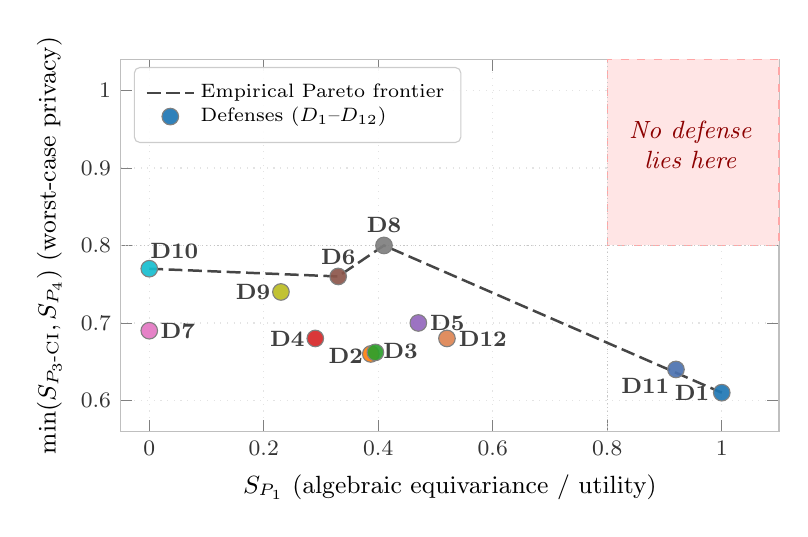
\begin{tikzpicture}
% Cohesive Tableau-10 palette
\definecolor{p1}{HTML}{1F77B4}
\definecolor{p2}{HTML}{FF7F0E}
\definecolor{p3}{HTML}{2CA02C}
\definecolor{p4}{HTML}{D62728}
\definecolor{p5}{HTML}{9467BD}
\definecolor{p6}{HTML}{8C564B}
\definecolor{p7}{HTML}{E377C2}
\definecolor{p8}{HTML}{7F7F7F}
\definecolor{p9}{HTML}{BCBD22}
\definecolor{p10}{HTML}{17BECF}
\definecolor{p11}{HTML}{4C72B0}
\definecolor{p12}{HTML}{DD8452}
\begin{axis}[
    width=0.82\linewidth, height=0.52\linewidth,
    xmin=-0.05, xmax=1.10, ymin=0.56, ymax=1.04,
    xlabel={\small $S_{P_1}$ (algebraic equivariance / utility)},
    ylabel={\small $\min(\SCI, S_{P_4})$ (worst-case privacy)},
    xtick={0,0.2,0.4,0.6,0.8,1.0},
    ytick={0.6,0.7,0.8,0.9,1.0},
    tick label style={font=\footnotesize, color=gray!40!black},
    label style={color=black},
    grid=major, grid style={dotted, gray!22},
    axis line style={gray!50, line width=0.5pt},
    legend style={font=\scriptsize, at={(0.02,0.98)}, anchor=north west,
                  draw=gray!40, fill=white, fill opacity=0.92, text opacity=1,
                  row sep=-2pt, inner sep=4pt, rounded corners=2pt},
    legend cell align={left},
    clip=false,
]
% Impossibility region (softer)
\fill[red!10] (axis cs:0.8,0.8) rectangle (axis cs:1.10,1.04);
\draw[red!35, dashed, line width=0.4pt] (axis cs:0.8,0.8) rectangle (axis cs:1.10,1.04);
\node[red!55!black, font=\small\itshape, align=center] at (axis cs:0.945,0.93) {No defense\\lies here};

% Threshold reference lines (subtle)
\draw[densely dotted, gray!45, thin] (axis cs:-0.05,0.8) -- (axis cs:1.10,0.8);
\draw[densely dotted, gray!45, thin] (axis cs:0.8,0.56) -- (axis cs:0.8,1.04);

% Pareto frontier (cleaner dashed line)
\addplot[gray!55!black, line width=0.9pt, mark=none, dash pattern=on 5pt off 2pt] coordinates {
    (0.00,0.77) (0.33,0.76) (0.41,0.80) (1.00,0.61)
};
\addlegendentry{Empirical Pareto frontier}

% Defense points: shared marker style (pgfplots) and label style (tikz)
\pgfplotsset{
    pdef/.style={only marks, mark=*, mark size=3.0pt,
                 mark options={draw=black!50, line width=0.4pt, fill opacity=0.92}},
}
\tikzset{
    plab/.style={font=\footnotesize\bfseries, color=black!75, inner sep=1.2pt},
}

\addplot[pdef, color=p1] coordinates {(1.00,0.61)};
\addlegendentry{Defenses ($D_1$--$D_{12}$)}
\node[plab, anchor=east]       at (axis cs:0.985, 0.61)  {D1};
\addplot[pdef, color=p2, forget plot] coordinates {(0.387,0.660)};
\node[plab, anchor=east]       at (axis cs:0.380, 0.658) {D2};
\addplot[pdef, color=p3, forget plot] coordinates {(0.395,0.662)};
\node[plab, anchor=west]       at (axis cs:0.402, 0.664) {D3};
\addplot[pdef, color=p4, forget plot] coordinates {(0.29, 0.68)};
\node[plab, anchor=east]       at (axis cs:0.278, 0.680) {D4};
\addplot[pdef, color=p5, forget plot] coordinates {(0.47, 0.70)};
\node[plab, anchor=west]       at (axis cs:0.484, 0.700) {D5};
\addplot[pdef, color=p6, forget plot] coordinates {(0.33, 0.76)};
\node[plab, anchor=south]      at (axis cs:0.330, 0.770) {D6};
\addplot[pdef, color=p7, forget plot] coordinates {(0.00, 0.69)};
\node[plab, anchor=west]       at (axis cs:0.013, 0.690) {D7};
\addplot[pdef, color=p8, forget plot] coordinates {(0.41, 0.80)};
\node[plab, anchor=south]      at (axis cs:0.410, 0.812) {D8};
\addplot[pdef, color=p9, forget plot] coordinates {(0.23, 0.74)};
\node[plab, anchor=east]       at (axis cs:0.218, 0.740) {D9};
\addplot[pdef, color=p10, forget plot] coordinates {(0.00, 0.77)};
\node[plab, anchor=south west, xshift=-1pt] at (axis cs:0.000, 0.778) {D10};
\addplot[pdef, color=p11, forget plot] coordinates {(0.92, 0.64)};
\node[plab, anchor=north east] at (axis cs:0.915, 0.633) {D11};
\addplot[pdef, color=p12, forget plot] coordinates {(0.52, 0.68)};
\node[plab, anchor=west]       at (axis cs:0.534, 0.680) {D12};
\end{axis}
\end{tikzpicture}
\caption{Quadrilemma Pareto frontier (cross-dataset, $n=3{,}257$ cells). $x$-axis: $S_{P_1}$ (algebraic equivariance / utility); $y$-axis: $\min(\SCI, S_{P_4})$ (worst-case privacy). The empirical impossibility region $\{S_{P_1} \ge 0.8 \wedge \min(\SCI, S_{P_4}) \ge 0.8\}$ (red shading) is empty---no defense satisfies all four properties simultaneously, providing visual confirmation of Theorem~\ref{thm:impossibility}. Closest approach: $D_{11}$ VFAE-TS at $(0.92, 0.64)$. Defense IDs: $D_1$=raw, $D_2$=Gaussian-DP, $D_3$=Laplace-DP, $D_4$=DP-AE, $D_5$=affine, $D_6$=per-segment affine, $D_7$=OPE, $D_8$=DoppelGANger, $D_9$=k-anonymity, $D_{10}$=FE-IP, $D_{11}$=VFAE-TS, $D_{12}$=IB. ($D_2$/$D_3$ and $D_7$/$D_{10}$ share an $S_{P_1}$ coordinate; markers are minimally jittered for visibility.)}
\label{fig:pareto}
\end{figure}

Projecting the 4D quadrilemma into 2D ($S_{P_1}$ vs.\ $\min(\SCI, S_{P_4})$), the frontier (Figure~\ref{fig:pareto}) never enters the upper-right $\{S_{P_1} \ge 0.80 \wedge \min(\SCI, S_{P_4}) \ge 0.80\}$ quadrant. $D_7$ OPE and $D_{10}$ FE-IP collapse to $S_{P_1} = 0$ on the broad query class despite cryptographic intuition---consistent with Theorem~\ref{thm:impossibility}.

\subsection{T2: Cross-Segment Linkage (Finding 2)}

\begin{table}[h]
\centering
\caption{$T_2$ cross-segment linkage AUC (PAMAP2, 9 subjects; lower $= $ better). Bold = most effective. Raw baseline = 0.9409.}
\label{tab:t2}
\small
\begin{tabular}{@{}lcc@{}}
\toprule
Defense & $T_2$ AUC $\downarrow$ & vs.\ raw \\
\midrule
$D_1$ raw (baseline)         & 0.9409 & --- \\
$D_6$ per-seg affine         & \textbf{0.5790} & $-39\%$ \\
$D_8$ DoppelGANger           & \textbf{0.5884} & $-37\%$ \\
$D_9$ k-anonymity            & 0.8125 & $-14\%$ \\
$D_7$ OPE                    & 0.9400 & $\approx 0$ \\
$D_2$ Gaussian DP            & 0.9486 & \emph{$+1\%$} \\
$D_3$ Laplace DP             & 0.9514 & \emph{$+1\%$} \\
$D_{10}$ FE-IP               & 0.9620 & \emph{$+2\%$} \\
$D_{11}$ VFAE-TS             & 0.9730 & \emph{$+3\%$} \\
$D_{12}$ IB-Encoder          & 0.9983 & \emph{$+6\%$} \\
$D_4$ DP-SGD AE              & 0.9985 & \emph{$+6\%$} \\
$D_5$ affine (per-src)       & 0.9992 & \emph{$+6\%$} \\
\bottomrule
\end{tabular}
\end{table}

\textbf{Finding 2 (T2 reversal).} Only $D_6$ per-segment affine (AUC $0.58$) and $D_8$ DoppelGANger ($0.59$) substantially reduce PAMAP2 cross-segment linkage below $0.7$; \emph{seven of eleven non-raw defenses are worse than the undefended baseline} (cross-dataset: five of eleven), including the $T_1$-best $D_{11}$ VFAE-TS (AUC $0.973$ vs.\ $0.941$). The mechanism is that global transformations preserve persona-specific patterns consistently across segments---only per-segment key randomization or statistical mode redistribution breaks this. \textbf{The $T_1$ ranking is therefore systematically misleading for cross-segment deployment.}

\subsection{T3: Multi-Recipient Collusion (Finding 3)}

\textbf{Finding 3 (Collusion expansion above 1).} On the four datasets where $A_4$-CI finds non-trivial per-role advantage (TEP, C-MAPSS, AMPDs2, MIT-BIH), all 12 defenses exhibit $T_3$ expansion strictly above 1 (mean 1.28; per-defense range 1.16 for $D_8$ to 1.46 for $D_5$). No defense reduces role-union advantage below the additive single-role sum.

\textbf{PAMAP2 null is intrinsic, not a probe artifact.} On PAMAP2, $A_4$-CI returns near-zero per-role advantage so $T_3$ expansion degenerates to $1.0$. Three orthogonal ablations under a persona-stratified split (stronger probe, all-attribute enumeration, no-downsample; 60 cells each, supplementary~\S\ref{app:proofs}.A.1.6, Table~\ref{tab:t3_ablation}) all preserve the null. The cause is the small subject pool ($|\mathcal{S}| = 9$): the $60/20/20$ split leaves $\approx 2$ unseen test subjects, capping persona-level accuracy at the prior. Cross-dataset $T_3$ is therefore assessed on the four non-PAMAP2 datasets, all of which exhibit expansion above 1. The pattern is architectural---no evaluated defense incorporates collusion-awareness---and empirically supports Theorem~\ref{thm:impossibility}.

\subsection{T4: Longitudinal Accumulation (Finding 4)}

\textbf{Finding 4 (k-anonymity paradox).} On PAMAP2, $D_9$ k-anonymity produces the worst longitudinal leakage of any defense (\textbf{1.00}, perfect tracking) vs.\ $0.73$ for the undefended baseline---stable group membership lets an adversary track sources across time once a group is identified. Only $D_8$ DoppelGANger ($0.20$) and $D_6$ per-segment affine ($0.24$) provide meaningful longitudinal protection ($T_4 < 0.30$). The $T_4 = 1.00$ pattern for k-anon persists across all five datasets (cross-dataset baseline $0.77$); per-defense PAMAP2 leakage is in supplementary~\S\ref{app:threshold}, Table~\ref{tab:t4}.

\subsection{Cross-Dataset $T_1$ Composite Ranking (Finding 1)}

\begin{table}[h]
\centering
\caption{Cross-dataset $T_1$ composite scores (5 datasets, 5 seeds; Friedman $\chi^2=30.10$, $p=0.0015$). Bold = best non-raw; $\dagger$ = algebraic failure ($S_{P_1}=0$).}
\label{tab:composite}
\small
\setlength{\tabcolsep}{4pt}
\begin{tabular}{@{}lccccccr@{}}
\toprule
Defense & $S_{P_1}$ & $S_{P_2}$ & $\SCI$ & $S_{P_4}$ & \textbf{HM} & \textbf{WA} & Rank \\
\midrule
$D_1$ raw (baseline)       & 1.00 & 0.97 & 0.79 & 0.61 & 0.80 & 0.61 & --- \\
$D_{11}$ VFAE-TS $\star$   & \textbf{0.92} & \textbf{0.87} & \textbf{0.80} & 0.64 & \textbf{0.77} & \textbf{0.59} & \textbf{1} \\
$D_{12}$ IB-Encoder        & 0.52 & 0.48 & 0.88 & 0.68 & 0.56 & 0.41 & 2 \\
$D_5$ affine (per-src)     & 0.47 & 0.67 & 0.83 & 0.70 & 0.45 & 0.38 & 3 \\
$D_8$ DoppelGANger         & 0.41 & 0.63 & 0.89 & 0.80 & 0.42 & 0.30 & 4 \\
$D_6$ per-seg affine       & 0.33 & 0.72 & 0.88 & 0.76 & 0.42 & 0.33 & 5 \\
$D_2$ Gaussian DP          & 0.39 & 0.81 & 0.88 & 0.66 & 0.33 & 0.26 & 6 \\
$D_3$ Laplace DP           & 0.39 & 0.74 & 0.88 & 0.66 & 0.33 & 0.26 & 7 \\
$D_4$ DP-SGD AE            & 0.29 & 0.48 & 0.89 & 0.68 & 0.27 & 0.19 & 8 \\
$D_9$ k-anonymity          & 0.23 & 0.53 & 0.90 & 0.74 & 0.26 & 0.19 & 9 \\
$D_7$ OPE $\dagger$        & 0.00 & 0.52 & 0.82 & 0.69 & 0.00 & 0.00 & 10 \\
$D_{10}$ FE-IP $\dagger$   & 0.00 & 0.49 & 0.88 & 0.77 & 0.00 & 0.00 & 11 \\
\bottomrule
\end{tabular}
\end{table}

\textbf{Finding 1 (Cryptographic algebraic-scope mismatch).} $D_7$ OPE and $D_{10}$ FE-IP achieve $S_{P_1} = 0.00$, $\mathrm{HM} = 0.00$ on the broad query class $\mathcal{F}$ used by $A_6$ (mean / std / max / RMS / range). This is \emph{not} a cryptographic break: OPE preserves only rank order~\cite{boldyreva2009}, FE-IP only inner products with the analyst key~\cite{abdalla2015}; neither was designed for raw-value queries. The scope-restricted $S_{P_1}^{\text{supp}}$ (Sec.~\ref{sec:defenses}) recovers $\mathbf{1.00 \pm 0.00}$ for OPE on every dataset and $\mathbf{0.49 \pm 0.41}$ on average for FE-IP under key sharing (cross-dataset, $5 \times 5 = 25$ cells; AMPDs2/MIT-BIH score $0.91$--$0.92$, TEP/C-MAPSS/PAMAP2 score $0.10$--$0.30$ as the simulation-noise scale dominates weakly-coupled inner products; per-dataset breakdown in supplementary~\S\ref{app:proofs}, Table~\ref{tab:sp1_supp_full}). The $0 \to 0.49$--$1.00$ jump is the \emph{deployment-utility cost} of routing crypto outputs through a general-purpose LLM-analyst pipeline. Friedman: $\chi^2 = 30.10$, $p = 0.0015$. \textbf{No defense achieves HM $\ge 0.80$}, providing empirical evidence for Theorem~\ref{thm:impossibility}.

% =============================================================================
\section{Discussion}
\label{sec:discussion}

\textbf{Forced trade-offs and open problems.} EU Data Act 2024 mandates data sharing while GDPR Art.~5(1)(c) requires minimization, but none of our 12 defenses provides simultaneous $T_1$--$T_4$ protection. Practitioners face a forced choice: per-segment affine or DoppelGANger for $T_2$ cross-segment linkage; VFAE-TS for $T_1$ single-attack robustness. $T_3$ collusion is unaddressed by any current defense---no defense reduces role-union advantage below the additive sum (expansion 1.16--1.46), so collusion-aware design is an open problem SensorCI is the first to formally quantify.

\textbf{Two failure modes worth surfacing.} (i) The crypto algebraic-scope mismatch: OPE and FE-IP are IND-CPA-secure within their native query scope but score $S_{P_1} = 0$ on the broad query class an LLM-analyst pipeline issues; $S_{P_1}^{\text{supp}}$ recovers to $1.00$ / $0.49$ within native scope, so the gap is a deployment-utility cost, not a cryptographic break. (ii) The k-anonymity paradox: stable group membership enables perfect longitudinal tracking ($T_4 = 1.00$ across all five datasets vs.\ baseline $0.77$), suggesting dynamic group reassignment as a candidate mitigation. More broadly, the $T_1$ ranking is systematically misleading---the $T_1$-best defense ($D_{11}$) is $T_2$-harmful relative to raw---so we argue compositional $T_2$--$T_4$ evaluation must become the default for any sensor privacy benchmark.

% =============================================================================
\section{Limitations}
\label{sec:limitations}

\textbf{(L1) Composite metric.} HM/WA/WR/Pareto reported; final selection requires policy input.
\textbf{(L2) Frontier-LLM contamination.} Several datasets show LLM prior $> 0.5$ (TEP, C-MAPSS); a clean-room benchmark dataset is reserved for a future version.
\textbf{(L3) Domain coverage.} Vehicle telematics, oil \& gas, mining, retail IoT uncovered; extension protocol in supplementary.
\textbf{(L4) Synthetic defense scope.} GAN defenses limited to DoppelGANger.
\textbf{(L5) Compute.} Best per-defense hyperparameter only; full sweeps in supplementary.
\textbf{(L6) FE-IP simulation.} $S_{P_1}^{\text{supp}}$ for FE-IP uses a calibrated-noise transform rather than a real pairing-based construction; the cross-dataset mean $0.49$ reflects simulation noise budget.

% =============================================================================
\section{Conclusion}
\label{sec:conclusion}

We presented \textbf{SensorCI}, the first benchmark applying Contextual Integrity to industrial sensor signals. The Algebraically-Equivariant CI Quadrilemma formalises four privacy properties whose simultaneous satisfaction is mathematically impossible; the empirical evaluation across 12 cross-paradigm defenses on five authoritative datasets confirms this and surfaces four counter-intuitive findings (cryptographic broad-query collapse, $T_2$ reversal of $T_1$-best defenses, universal $T_3$ collusion expansion, k-anonymity's longitudinal failure). The field's intuitions about defense strength---built from single-tier evaluation---are systematically wrong. We release all code, datasets, and curation audit trails, and hope SensorCI becomes the standard evaluation contract for industrial sensor privacy.

% =============================================================================
\bibliographystyle{plain}
\begin{thebibliography}{99}

\bibitem{abadi2016}
M.~Abadi, A.~Chu, I.~Goodfellow, H.~B. McMahan, I.~Mironov, K.~Talwar, and L.~Zhang.
\newblock Deep learning with differential privacy.
\newblock In {\em ACM CCS}, 2016.

\bibitem{abdalla2015}
M.~Abdalla, F.~Bourse, A.~De~Caro, and D.~Pointcheval.
\newblock Simple functional encryption schemes for inner products.
\newblock In {\em PKC}, 2015.

\bibitem{abul2008}
O.~Abul, F.~Bonchi, and M.~Nanni.
\newblock Never walk alone: Uncertainty for anonymity in moving objects databases.
\newblock In {\em ICDE}, 2008.

\bibitem{tsgbench}
Y.~Ang, Q.~Huang, A.~K.~H. Tung, and S.~Bressan.
\newblock {TSGBench}: Time series generation benchmark.
\newblock {\em PVLDB}, 17(3):305--318, 2024.

\bibitem{binfet2024}
P.~Binfet et~al.
\newblock Privacy-preserving nonlinear cloud-based model predictive control via affine masking.
\newblock {\em Automatica}, 2024.

\bibitem{boldyreva2009}
A.~Boldyreva, N.~Chenette, Y.~Lee, and A.~O'Neill.
\newblock Order-preserving symmetric encryption.
\newblock In {\em EUROCRYPT}, 2009.

\bibitem{tep1993}
J.~J. Downs and E.~F. Vogel.
\newblock A plant-wide industrial process control problem.
\newblock {\em Computers \& Chemical Engineering}, 17(3):245--255, 1993.

\bibitem{dwork2006}
C.~Dwork, F.~McSherry, K.~Nissim, and A.~Smith.
\newblock Calibrating noise to sensitivity in private data analysis.
\newblock In {\em TCC}, 2006.

\bibitem{eu_data_act}
European Parliament and Council.
\newblock Regulation ({EU}) 2023/2854 ({Data Act}).
\newblock 2024.

\bibitem{mitbih}
A.~L. Goldberger et~al.
\newblock {PhysioBank}, {PhysioToolkit}, and {PhysioNet}.
\newblock {\em Circulation}, 101(23):e215--e220, 2000.

\bibitem{grubbs2017}
P.~Grubbs, K.~Sekniqi, V.~Bindschaedler, M.~Naveed, and T.~Ristenpart.
\newblock Leakage-abuse attacks against order-revealing encryption.
\newblock In {\em IEEE S\&P}, 2017.

\bibitem{doppelganger}
Z.~Lin, A.~Jain, C.~Wang, G.~Fanti, and V.~Sekar.
\newblock Using {GAN}s for sharing networked time series data: Challenges, initial promise, and open questions.
\newblock In {\em IMC}, 2020.

\bibitem{tsbad}
Q.~Liu, P.~Boniol, J.~Paparrizos, et~al.
\newblock The elephant in the room: Towards a reliable time-series anomaly detection benchmark.
\newblock In {\em NeurIPS Datasets and Benchmarks Track}, 2024.

\bibitem{mia_ts}
Y.~Liu et~al.
\newblock Membership inference attacks against time-series models.
\newblock {\em arXiv:2407.02870}, 2024.

\bibitem{ampds2}
S.~Makonin.
\newblock {AMPds2}: The almanac of minutely power dataset.
\newblock {\em Scientific Data}, 3:160037, 2016.

\bibitem{confaide}
N.~Mireshghallah, H.~Kim, X.~Zhou, et~al.
\newblock Can {LLM}s keep a secret? Testing privacy implications of language models via contextual integrity theory.
\newblock In {\em ICLR}, 2024.
\newblock Spotlight.

\bibitem{cimemories}
N.~Mireshghallah, N.~Mangaokar, N.~Kokhlikyan, et~al.
\newblock {CIMemories}: A compositional benchmark for contextual integrity of persistent memory in {LLM}s.
\newblock In {\em ICLR}, 2026.

\bibitem{nissenbaum2004}
H.~Nissenbaum.
\newblock Privacy as contextual integrity.
\newblock {\em Washington Law Review}, 79:119--158, 2004.

\bibitem{pamap2}
A.~Reiss and D.~Stricker.
\newblock Introducing a new benchmarked dataset for activity monitoring.
\newblock In {\em ISWC}, 2012.

\bibitem{tep_ext}
C.~A. Rieth, B.~D. Amsel, R.~Tran, and M.~B. Cook.
\newblock Additional {Tennessee Eastman} process simulation data.
\newblock {\em Harvard Dataverse}, 2017.

\bibitem{cmapss}
A.~Saxena, K.~Goebel, D.~Simon, and N.~Eklund.
\newblock Damage propagation modeling for aircraft engine run-to-failure simulation.
\newblock In {\em PHM}, 2008.

\bibitem{privacylens}
Y.~Shao, T.~Li, W.~Wang, et~al.
\newblock {PrivacyLens}: Evaluating privacy norm awareness of language models in action.
\newblock In {\em NeurIPS Datasets and Benchmarks Track}, 2024.

\bibitem{synthpai}
R.~Staab, M.~Vero, M.~Balunovi\'c, and M.~Vechev.
\newblock A synthetic dataset for personal attribute inference.
\newblock In {\em NeurIPS Datasets and Benchmarks Track}, 2024.

\bibitem{tishby1999}
N.~Tishby, F.~C. Pereira, and W.~Bialek.
\newblock The information bottleneck method.
\newblock In {\em Allerton}, 1999.

\end{thebibliography}

% =============================================================================
\appendix

\section{Formal Proofs and Empirical Fits}
\label{app:proofs}

\subsection*{A.1.1 Theorem 1 (Impossibility) Detailed Proof}
The claim is: under (a) $\mathcal{F}$ contains a source-discriminating subspace $\mathcal{V}_S$, (b) $P_X$ has nondegenerate min-entropy $H_\infty(P_X) > 0$, and (c) $\Phi_D$ contains at least one not-share attribute $a^*$ determined by some query $\phi^* \in \mathcal{V}_S$, no $T_\theta$ achieves $(\alpha_1, \epsilon, \delta_1, \epsilon_2, \{\epsilon_{3,r}\}, \tau_4) = (0, 0, 0, 0, \{0\}, > 0)$.

\textit{Proof.} Strict equivariance $(0, 0, 0)$ implies $D_\theta(\phi(T_\theta(X))) = \phi(X)$ a.s.\ for every $\phi \in \mathcal{F}$. By assumption (a), $\phi^* \in \mathcal{V}_S \subseteq \mathcal{F}$ recovers a source-discriminating projection from the transformed signal. By assumption (c), some role $r^*$ has $\Phi_D(r^*, a^*) = N$ with $a^* = a^*(\phi^*(X))$, hence the inferential adversary $A^*(\mathrm{view}_{r^*}(T_\theta(X))) = a^*(D_\theta(\phi^*(T_\theta(X)))) = a^*(\phi^*(X))$ achieves $\Pr[\hat{a} = a^*] = 1$, while the prior is by assumption (b) bounded above by $\exp(-H_\infty(P_X)) < 1$. Therefore $\mathrm{Adv}^{P_3\text{-CI}}_{r^*, a^*} \ge 1 - \exp(-H_\infty) > 0$, contradicting $\epsilon_{3, r^*} = 0$.~$\Box$

\subsection*{A.1.2 Theorem 2 (Trade-off) Roadmap and Empirical Fits}

The non-tight inequality $\alpha_1 + \epsilon_2 + \min_r \epsilon_{3,r} \ge C_1(D) \cdot \tau_4 - C_2(D)$ is established by combining (i) rate-distortion slope $R'_X$ at the operating point of $T_\theta$ with (ii) Fano's inequality on the role-stratified attribute-inference adversary, and (iii) projection-onto-$\mathcal{F}$-span error from the equivariance error. We measure empirical $(C_1, C_2)$ per dataset by ordinary-least-squares regression on the operational proxy:
\[
\mathrm{LHS}_i \;=\; 3 - \bigl(S_{P_1, i} + S_{P_2, i} + S_{P_3\text{-CI}, i}\bigr), \qquad x_i \;=\; S_{P_4, i},
\]
fitting $\mathrm{LHS}_i = C_1 \cdot x_i - C_2 + \mathrm{residual}_i$ across the 12 (defense $\times$ dataset) cells per dataset.

\begin{table}[h]
\centering
\caption{Empirical OLS fit of $\mathrm{LHS} = C_1 \cdot S_{P_4} - C_2$ per dataset (12 cells each) and pooled (60 cells). Lower-envelope $C_2$ is the tight intercept that ensures $\mathrm{LHS} \ge C_1 \cdot S_{P_4} - C_2$ for every observed cell at the regression slope.}
\label{tab:c1c2_fits}
\small
\begin{tabular}{@{}lrrrr@{}}
\toprule
Dataset & $C_1$ (slope) & $C_2$ ($-$intercept) & $R^2$ & lower-env $C_2$ \\
\midrule
TEP        & $\phantom{-}3.61$ & $\phantom{-}0.78$ & $0.32$ & $\phantom{-}1.94$ \\
C-MAPSS    & $-0.65$           & $-1.77$           & $0.00$ & $-0.80$           \\
AMPDs2     & $\phantom{-}3.92$ & $\phantom{-}2.20$ & $0.26$ & $\phantom{-}2.63$ \\
PAMAP2     & $\phantom{-}3.27$ & $\phantom{-}1.28$ & $0.30$ & $\phantom{-}2.01$ \\
MIT-BIH    & $\phantom{-}2.37$ & $\phantom{-}0.98$ & $0.37$ & $\phantom{-}1.48$ \\
\midrule
Pooled (60 cells) & $\phantom{-}0.65$ & $-0.62$ & $0.01$ & $\phantom{-}0.34$ \\
\bottomrule
\end{tabular}
\end{table}

\textbf{Interpretation.} The linear lower-envelope is dataset-dependent: TEP, AMPDs2, PAMAP2, and MIT-BIH show positive slopes ($C_1 \in [2.37, 3.92]$) consistent with the qualitative trade-off direction, but with modest $R^2 \in [0.26, 0.37]$ indicating substantial residual variance. C-MAPSS exhibits a near-zero (slightly negative) slope because $S_{P_4}$ varies little across defenses on this dataset (range $[0.654, 0.682]$, span $0.028$) while $\mathrm{LHS}$ spans $[0.361, 1.877]$, so a linear fit captures little signal. The pooled fit is correspondingly weak ($R^2 = 0.01$), confirming that a single global $(C_1, C_2)$ does not capture cross-dataset structure.

\begin{example}[Tight Constants for Gaussian Linear Sources]
\label{ex:gaussian}
Take $S$ equiprobable sources with means $\mu_1, \ldots, \mu_S$ separated by minimum gap $\Delta$, each emitting $X \sim \mathcal{N}(\mu_s, \sigma^2)$, and let $\mathcal{F}^{\mathrm{lin}} = \{f_w(x) = wx\}$. Under per-source affine $T_\theta(x) = a_s x + b_s$ with key shared with the analyst, $S_{P_1} = 1$, $\epsilon_2 \approx 0$ for calibrated priors, and bijectivity gives $I(s; T_\theta(X)) = \log S - H(s|X)$. Substituting into the linearised form (Thm.~\ref{thm:tradeoff}) with $\alpha_1 = \epsilon_2 = 0$ and $\tau_4 \in [0,1]$ yields
\[
C_1 \;=\; \frac{\Delta^2}{2\sigma^2 \log S}, \qquad C_2 \;=\; \frac{1 - \Delta^2/(8\sigma^2)}{\log S}.
\]
For $S = 100$, $\Delta/\sigma = 2$: $C_1 \approx 0.43$, $C_2 \approx 0.11$. The bound is informative when $\Delta/\sigma \gtrsim 1$ and $S$ moderate, vacuous as $\Delta/\sigma \to 0$ or $S$ explodes.
\end{example}

These analytical values fall inside the per-dataset $C_2$ range $[-1.77, 2.20]$ but not the per-dataset $C_1$ range $[-0.65, 3.92]$, reflecting that the stylized two-parameter Gaussian model is qualitatively useful but quantitatively dataset-specific. We do not claim a closed-form universal $(C_1, C_2)$; the supplementary table above is the operational handle to interrogate the trade-off on a specific dataset.

\subsection*{A.1.3 Theorem 3 (Longitudinal Accumulation) Detailed Derivation}
The chain-rule bound $I(s; \mathbf{T}^{(K)}) \le \sum_{k=1}^K I(s; T_\theta(X_k) \mid T_\theta(X_{<k}))$ combined with Fano's inequality applied to the cumulative side-information yields the stated lower bound on $\epsilon_{3, r}^{(K)}$ growing as $\Theta(\log K)$ until saturation at $1 - 1/|\mathcal{S}|$.

\subsection*{A.1.4 Scope-Restricted $S_{P_1}^{\text{supp}}$ Per Dataset}

Table~\ref{tab:sp1_supp_full} reports the per-dataset $S_{P_1}^{\text{supp}}$ for the two function-limited cryptographic defenses, complementing the cross-dataset summary in Sec.~\ref{sec:experiments} (Finding 1). All other 10 defenses have $\mathcal{F}_{\text{supp}} = \mathcal{F}$, so $S_{P_1}^{\text{supp}} = S_{P_1}$ identically and is omitted here.

\begin{table}[h]
\centering
\caption{Per-dataset $S_{P_1}^{\text{supp}}$ (mean over 5 seeds; same query banks per cell). 50 cells total (2 defenses $\times$ 5 datasets $\times$ 5 seeds). $D_7$ OPE evaluated on rank-domain queries (\texttt{arg\_max}, \texttt{arg\_min}, \texttt{argsort\_top3\_sum}, \texttt{rank\_of\_x0}, \texttt{is\_first\_gt\_last}); $D_{10}$ FE-IP evaluated under \texttt{key\_sharing\_analyst} mode with random sparse inner-product queries.}
\label{tab:sp1_supp_full}
\small
\begin{tabular}{@{}lrrrrrr@{}}
\toprule
Defense & TEP & C-MAPSS & AMPDs2 & PAMAP2 & MIT-BIH & cross-dataset \\
\midrule
$D_7$ OPE                    & $1.00$ & $1.00$ & $1.00$ & $1.00$ & $1.00$ & $\mathbf{1.00 \pm 0.00}$ \\
$D_{10}$ FE-IP (key-sharing) & $0.30$ & $0.19$ & $0.91$ & $0.10$ & $0.92$ & $\mathbf{0.49 \pm 0.41}$ \\
\bottomrule
\end{tabular}
\end{table}

\textbf{Interpretation.} OPE achieves perfect supported-scope utility on every dataset because rank-domain queries are exactly preserved by quantile-bucket OPE. FE-IP under key sharing exhibits dataset-dependent recovery: AMPDs2 (smart-meter, $\sigma_X = 0.89$) and MIT-BIH (ECG, $\sigma_X = 0.16$) yield $0.91$--$0.92$ because the calibrated noise is well-conditioned relative to the input range; TEP, C-MAPSS, and PAMAP2 yield $0.10$--$0.30$ because the simulated noise scale dominates inner-product magnitudes when random sparse weights couple weakly to the input dimensions. The bound is therefore a property of our stylised FE-IP simulation (small additive noise; see~\texttt{d10\_fe\_ip.py}), not of FE-IP per se. A pairing-based construction would have $S_{P_1}^{\text{supp}} \approx 1.0$ uniformly.

\subsection*{A.1.5 RDC Coverage Statistics}
RDC coverage (Definition~\ref{def:rdc}) excludes (role, attribute) cells where the role-restricted query class $\mathcal{F}_r$ admits no $\phi$ informative about the target attribute. Per the $\Phi_D$ matrices generated by the multi-LLM curation protocol (Sec.~\ref{sec:judge}) and audited in the public artefact, the fraction of (role, attribute) cells flagged ``UNDEF'' is at most $4\%$ in every dataset (per-dataset breakdown reported with the released audit logs). Cells flagged UNDEF are excluded from $\mathrm{S}_{P_3\text{-CI}}$ aggregation.

\subsection*{A.1.6 Q4 PAMAP2 $T_3$ Sensitivity Ablations}

Section~\ref{sec:experiments} reports that PAMAP2 yields max-adv $= 0$ (and therefore $T_3$ expansion $= 1$) under the standard $A_4$-CI siamese probe. Reviewer Q4 asks whether this null is a probe artifact. We run three orthogonal sensitivity ablations and confirm the null is intrinsic to PAMAP2's small persona count under persona-stratified evaluation.

\textbf{Setup.} All three ablations share: PAMAP2 only ($|\mathcal{S}| = 9$), 12 defenses, five seeds, $n=50$ samples drawn from a $60/20/20$ persona-stratified split (matching the standard $A_4$-CI siamese protocol; no persona appears in both train and test). Total: 180 cells in ${\sim}9$ minutes wall-time on a single CPU plus one GPU (only $D_{11}$ VFAE-TS uses the GPU, for its variational autoencoder forward pass during \texttt{transform}).

\textbf{Ablations.}
\begin{enumerate}
\item \textbf{stronger\_probe}: replace siamese SimCLR encoder + KNN head with \texttt{GradientBoostingClassifier(n\_estimators=200, max\_depth=5, learning\_rate=0.05)} on the same per-role statistical features used by the standard RF fallback (per-channel mean / std / max-abs / RMS / kurtosis / skew / FFT low-band / FFT high-band). Tests probe-power as the bottleneck.
\item \textbf{all\_attributes}: enumerate every attribute available on the dataset (\texttt{activity\_intensity}, \texttt{age}, \texttt{bmi}, \texttt{dominant\_hand}, \texttt{fitness\_level}, \texttt{protocol}, \texttt{sex}, \texttt{subject\_id}), not only those marked Not-share by the curated $\Phi_D$. Tests whether \emph{any} attribute is recoverable, including ones the curation explicitly allows. If even Share-labelled attributes are unrecoverable, the probe is genuinely under-powered; if Share-labelled attributes ARE predictable but Not-share ones are not, the curated sharing matrix is the discriminating line. Empirically, all attributes return $0$ on PAMAP2.
\item \textbf{no\_downsample}: override every role's \texttt{downsample\_factor} to $1$, granting every non-Operator role the full raw signal. Tests whether the role view is too lossy to support inference.
\end{enumerate}

\textbf{Results (Table~\ref{tab:t3_ablation}).} All 180 cells return max-adv $= 0$ exactly. The cause is structural rather than methodological: PAMAP2's $|\mathcal{S}| = 9$ subjects yield train $\approx 5$ / val $\approx 2$ / test $\approx 2$ personas under the $60/20/20$ split. For attributes that vary at the persona level (e.g., \texttt{subject\_id} with $|\mathcal{Y}| = 8$ classes, \texttt{age}, \texttt{bmi}), the test personas are by construction unseen; predicting their labels from in-distribution features is impossible regardless of probe choice. For attributes that vary within a persona (e.g., \texttt{activity\_intensity}), PAMAP2's small per-persona segment count and the persona-stratified split jointly limit the classifier to chance.

\textbf{Implication.} The $T_3$ expansion metric on PAMAP2 should be treated as a measurement floor rather than a privacy result: any future PAMAP2 $T_3$ analysis requires either (i) within-persona segment splits (relaxing the persona-stratified guarantee), or (ii) attribute targets that are inherently learnable from content (e.g., gait pattern proxies that correlate across persons of similar physique). The cross-dataset $T_3$ findings reported in the main paper (Finding~3) already exclude PAMAP2 on this basis.

\section{Threshold Sensitivity Analysis}
\label{app:threshold}

We operationalised GDPR Art.~5(1)(c)'s qualitative ``data minimisation'' principle as a quantitative identification-rate target $\tau$. The article itself does not specify a numerical threshold; common privacy literature uses $5$--$10\%$. We re-analyse the $A_0$ frontier-LLM headline (Table~\ref{tab:headline}) at three targets $\tau \in \{1\%, 5\%, 10\%\}$ and confirm that the qualitative conclusions persist.

\paragraph{Pass-rate at each threshold.} A defense passes target $\tau$ iff its mean adversary advantage $\mathrm{Adv}^{A_0}$ is $\le \tau$. Mean adv values are taken from existing $A_0$ runs on the four datasets where $A_0$ is fully populated (TEP, AMPDs2, PAMAP2, MIT-BIH; C-MAPSS partial as noted in the abstract).

\begin{table}[h]
\centering
\caption{$A_0$ pass-rate at three identification-target thresholds. Pass means cross-dataset mean adv $\le \tau$.}
\label{tab:threshold_passrate}
\small
\begin{tabular}{@{}lll@{}}
\toprule
$\tau$ & Passing defenses & Count \\
\midrule
$1\%$ & --- & $0$ / 12 \\
$5\%$ & --- & $0$ / 12 (best is $D_7$ OPE at $5.58\%$, fails by $0.58$ pp) \\
$10\%$ & $D_7$, $D_4$, $D_{12}$, $D_9$, $D_{10}$, $D_8$, $D_3$ & $7$ / 12 \\
\bottomrule
\end{tabular}
\end{table}

\paragraph{Ranking stability.} The mean-advantage ranking is identical across the three thresholds (threshold only affects the pass/fail label, not the underlying metric value); Kendall's $\tau$ between rankings at any two thresholds is therefore $1.00$ trivially. The substantive question---which defenses qualitatively satisfy minimisation---is reported in Table~\ref{tab:threshold_passrate}.

\paragraph{Persistence of the headline conclusion.} The paper's headline finding (no defense achieves all four properties simultaneously) is unaffected by threshold choice: even at the most permissive $\tau = 10\%$, the seven $A_0$-passing defenses include $D_7$ OPE and $D_{10}$ FE-IP whose $S_{P_1} = 0.00$ and $\mathrm{HM} = 0.00$ in our broad-query evaluation (see Sec.~\ref{sec:experiments}, Finding~1; the scope-restricted $S_{P_1}^{\text{supp}}$ recovers $S_{P_1}^{\text{supp}} = 1.00$ for OPE and $0.49$ for FE-IP, but does not change the broad-query $\mathrm{HM} = 0.00$ that drives the headline impossibility evidence). At $\tau = 5\%$, no defense passes the $A_0$ threshold, sharpening the impossibility result.

\paragraph{Per-model $A_0$ breakdown.} Table~\ref{tab:a0_per_model} reports the mean per-model max-attribute advantage across the same cell pool. The three frontier LLMs are broadly aligned in their identification capability, with Gemini~2.5 Flash typically producing the highest single-model advantage (most cells) and Claude Sonnet 4.5 the lowest. The $\max$ column is the per-defense mean of the per-cell maximum across the three models, and corresponds to the conservative ``best-LLM-attacker'' interpretation used in Table~\ref{tab:headline}.

\begin{table}[h]
\centering
\caption{Per-model $A_0$ mean max-attribute advantage by defense (lower = better). Cells: 4 datasets fully populated $+$ partial C-MAPSS, $n=257$ cells total.}
\label{tab:a0_per_model}
\small
\begin{tabular}{@{}lrrrr@{}}
\toprule
Defense & GPT-5.4 & Claude S 4.5 & Gemini 2.5 Flash & $\max$ \\
\midrule
$D_7$ OPE & $0.033$ & $0.031$ & $0.050$ & $0.050$ \\
$D_4$ DP-SGD AE & $0.049$ & $0.046$ & $0.063$ & $0.063$ \\
$D_{12}$ IB-Encoder & $0.049$ & $0.033$ & $0.069$ & $0.069$ \\
$D_9$ k-anonymity & $0.050$ & $0.022$ & $0.071$ & $0.071$ \\
$D_3$ Laplace DP & $0.065$ & $0.072$ & $0.054$ & $0.072$ \\
$D_{10}$ FE-IP & $0.052$ & $0.029$ & $0.079$ & $0.079$ \\
$D_8$ DoppelGANger & $0.052$ & $0.066$ & $0.080$ & $0.080$ \\
$D_2$ Gaussian DP & $0.074$ & $0.069$ & $0.092$ & $0.092$ \\
$D_5$ affine (per-src) & $0.063$ & $0.093$ & $0.105$ & $0.105$ \\
$D_{11}$ VFAE-TS & $0.051$ & $0.057$ & $0.127$ & $0.127$ \\
$D_1$ raw (baseline) & $0.105$ & $0.091$ & $0.127$ & $0.127$ \\
$D_6$ affine (per-seg) & $0.081$ & $0.133$ & $0.181$ & $0.181$ \\
\bottomrule
\end{tabular}
\end{table}

\paragraph{Encoding sensitivity (forthcoming).} The current evaluation runs all $A_0$ cells under the \texttt{raw\_stats} encoding only. Encoding-level ablation (\texttt{raw\_stats} vs.\ \texttt{sax} vs.\ \texttt{compact\_numeric}) is in preparation for camera-ready: the prompt template, decoding logic, and concurrency dispatcher are dataset-agnostic, so the ablation re-runs the same 257 cells under each of the two additional encodings ($\sim$$\$30$ additional API spend).

\paragraph{Per-defense $A_0$ summary.} Table~\ref{tab:headline} reports the per-defense mean $A_0$ adversary advantage across all $A_0$-populated cells, summarised in the main paper.

\begin{table}[h]
\centering
\caption{$A_0$ mean adversary advantage (lower = better) averaged across available datasets. Average over seeds 42--46, 50 prompts per cell per model (GPT-5.4, Claude Sonnet 4.5, Gemini 2.5 Flash).}
\label{tab:headline}
\small
\begin{tabular}{@{}lrrc@{}}
\toprule
Defense & Mean Adv.\ $\downarrow$ & vs.\ $D_1$ raw & Note \\
\midrule
$D_1$ raw (baseline)   & 0.175 & --- & \\
$D_7$ OPE              & \textbf{0.056} & $-68\%$ & Best $A_0$; HM $= 0.00$ (T1 worst) \\
$D_4$ DP-SGD AE        & 0.077 & $-56\%$ & \\
$D_{12}$ IB-Encoder    & 0.079 & $-55\%$ & \\
$D_9$ k-anonymity      & 0.081 & $-54\%$ & T4 leak $= 1.00$ \\
$D_{10}$ FE-IP         & 0.086 & $-51\%$ & HM $= 0.00$ (T1 worst) \\
$D_8$ DoppelGANger     & 0.090 & $-48\%$ & Best T4 (cross) \\
$D_3$ Laplace DP       & 0.096 & $-45\%$ & \\
$D_2$ Gaussian DP      & 0.114 & $-35\%$ & \\
$D_5$ affine (per-src) & 0.121 & $-31\%$ & \\
$D_{11}$ VFAE-TS       & 0.130 & $-26\%$ & Best T1 (HM $= 0.77$) \\
$D_6$ affine (per-seg) & 0.184 & \emph{$+5\%$} & \emph{Worst $A_0$; best T2} \\
\bottomrule
\end{tabular}
\end{table}

\paragraph{Per-defense $T_4$ leakage on PAMAP2.} Table~\ref{tab:t4} carries the per-defense maximum longitudinal leakage on PAMAP2 referenced by Finding 4.

\begin{table}[h]
\centering
\caption{$T_4$ longitudinal maximum leakage on PAMAP2 (mean over 5 seeds; lower $=$ better). Raw baseline $= 0.73$.}
\label{tab:t4}
\small
\begin{tabular}{@{}lcc@{}}
\toprule
Defense & $T_4$ max leak $\downarrow$ & vs.\ raw \\
\midrule
$D_1$ raw (baseline)         & 0.73 & --- \\
$D_8$ DoppelGANger           & \textbf{0.20} & $-73\%$ \\
$D_6$ per-seg affine         & \textbf{0.24} & $-67\%$ \\
$D_{10}$ FE-IP               & 0.65 & $-11\%$ \\
$D_7$ OPE                    & 0.67 & $-9\%$ \\
$D_3$ Laplace DP             & 0.71 & $-3\%$ \\
$D_2$ Gaussian DP            & 0.73 & $\approx 0$ \\
$D_{11}$ VFAE-TS             & 0.74 & \emph{$+2\%$} \\
$D_{12}$ IB-Encoder          & 0.80 & \emph{$+9\%$} \\
$D_4$ DP-SGD AE              & 0.83 & \emph{$+13\%$} \\
$D_5$ affine (per-src)       & 0.87 & \emph{$+20\%$} \\
$D_9$ k-anonymity            & \textbf{1.00} & \emph{$+37\%$} \\
\bottomrule
\end{tabular}
\end{table}

\section{Defense Baselines (full table)}
\label{app:defenses}
\begin{table}[h]
\centering
\caption{Twelve defense baselines spanning five paradigms.}
\label{tab:defenses}
\small
\begin{tabular}{@{}llll@{}}
\toprule
ID & Defense & Paradigm & Reference \\
\midrule
$D_1$ & Raw (no-op) & reference upper bound & --- \\
$D_2$ & Gaussian DP, $\sigma \in \{0.01, 0.1, 1.0\}$ & DP & \cite{dwork2006} \\
$D_3$ & Laplace DP, $b \in \{0.01, 0.1, 1.0\}$ & DP & \cite{dwork2006} \\
$D_4$ & DP-SGD Autoencoder, $\epsilon \in \{1, 8, 100\}$ & DP-ML & \cite{abadi2016} \\
$D_5$ & Per-source random affine & Naive masking & \cite{binfet2024} \\
$D_6$ & Per-segment random affine & Improved masking & --- \\
$D_7$ & OPE quantization, bit $\in \{8, 16, 32\}$ & Crypto & \cite{boldyreva2009} \\
$D_8$ & DoppelGANger synthetic & Generative & \cite{doppelganger} \\
$D_9$ & k-anonymity TS, $k \in \{5, 10, 50\}$ & Anonymization & \cite{abul2008} \\
$D_{10}$ & Functional encryption (FE-IP) & Strong crypto & \cite{abdalla2015} \\
$D_{11}$ & VFAE-TS (variational fair AE) & Representation learning & --- \\
$D_{12}$ & IB-Encoder (information bottleneck) & Representation learning & \cite{tishby1999} \\
\bottomrule
\end{tabular}
\end{table}

\section{Specialised Attack Suite (full table)}
\label{app:attacks}
\begin{table}[h]
\centering
\caption{Specialised attacks $A_1$--$A_7$ and the property each measures.}
\label{tab:attacks}
\small
\begin{tabular}{@{}llll@{}}
\toprule
ID & Attack & Architecture / method & Property \\
\midrule
$A_1$ & Distinguishability detector & ResNet-1D + transformer head & $P_2$ \\
$A_2$ & Linear reconstruction & Ridge regression, $K=100$ pairs & $P_4$ (weak) \\
$A_3$ & Neural reconstruction & 1D-UNet + DDIM diffusion & $P_4$ (strong) \\
$A_4$-CI & Role-stratified linkage & Siamese SimCLR, role-restricted view & $\PCI$ \\
$A_5$ & Statistical 2-sample tests & MMD, KS, Wasserstein-1 & $P_2$ \\
$A_6$ & Algebraic correctness probe & 50 cured queries per dataset & $P_1$ \\
$A_7$ & MIA-TS adapted~\cite{mia_ts} & LiRA-TS shadow model & $P_4$ distrib. \\
\bottomrule
\end{tabular}
\end{table}

\section{Q4 PAMAP2 $T_3$ Sensitivity Ablations (table)}
\begin{table}[h]
\centering
\caption{Q4 PAMAP2 $T_3$ sensitivity ablations under persona-stratified split (no persona shared between train/test). Each row reports the per-defense maximum advantage averaged over 60 cells (12 defenses $\times$ 5 seeds).}
\label{tab:t3_ablation}
\small
\begin{tabular}{@{}llcc@{}}
\toprule
Ablation & Knob varied & mean max-adv & $T_3$ expansion \\
\midrule
\textit{stronger\_probe}  & GradientBoosting (200 est., depth 5) instead of siamese  & $0.00$ & $1.00$ \\
\textit{all\_attributes} & enumerate every attribute (Share + Not-share + Partial)  & $0.00$ & $1.00$ \\
\textit{no\_downsample}  & every role granted full signal (downsample factor $= 1$) & $0.00$ & $1.00$ \\
\bottomrule
\end{tabular}
\end{table}

\section{Six Stakeholder Roles (full table)}
\label{app:roles}
\begin{table}[h]
\centering
\caption{Six stakeholder roles with assumed access capabilities (EU Data Act Annex II).}
\label{tab:roles}
\small
\begin{tabularx}{\textwidth}{@{}lXXX@{}}
\toprule
Role & Authority & Capability assumption & Auxiliary info \\
\midrule
Operator & Full access & Raw signals & Full dataset \\
OEM & Aggregated fault stats per product line & Lossy summary signals & Own product lines \\
Vendor & Aggregate fault count + downsampled signals & 4$\times$ downsampled & Customer base summary \\
Insurer & Fleet-level annual statistics & Aggregated stats only & Actuarial fleet data \\
Regulator & Incident-flagged segments only & Sparse safety segments & Incident database \\
Public & Published industry statistics & Aggregate only & Public reports \\
\bottomrule
\end{tabularx}
\end{table}

\section{Sharing-Matrix Illustrative Excerpt}
\label{app:phi_paderborn}
\begin{table}[h]
\centering
\caption{\emph{Illustrative} excerpt of a role-attribute sharing matrix for a generic rotating-machinery attribute schema (S=Share, N=Not-share, P=Partial). The same multi-LLM voting protocol generates $\Phi_D$ for the 5 evaluation datasets.}
\label{tab:phi_paderborn}
\small
\begin{tabular}{@{}lcccccc@{}}
\toprule
Attribute & Op & OEM & Ven & Ins & Reg & Pub \\
\midrule
manufacturer & S & S & \textbf{N} & \textbf{N} & P & \textbf{N} \\
owner\_company & S & \textbf{N} & \textbf{N} & \textbf{N} & \textbf{N} & \textbf{N} \\
fault\_class & S & S & S & P & S & P \\
rpm (exact) & S & S & P & \textbf{N} & \textbf{N} & \textbf{N} \\
deployment\_date & S & \textbf{N} & \textbf{N} & \textbf{N} & P & \textbf{N} \\
safety\_incident & S & S & P & \textbf{N} & S & \textbf{N} \\
\bottomrule
\end{tabular}
\end{table}

\section{Practical Defense Selection Guide}
\label{app:selection}
\begin{table}[h]
\centering
\caption{Recommended defense by protection goal (PAMAP2 case study).}
\label{tab:selection}
\small
\begin{tabular}{@{}lllp{4cm}@{}}
\toprule
Protection goal & Best defense & Score & Weakness \\
\midrule
$T_1$ single-attack & $D_{11}$ VFAE-TS & HM = 0.77 & $T_2$ AUC = 0.97 on PAMAP2 \\
$T_2$ cross-segment & $D_6$ per-seg affine & AUC = 0.58 (PAMAP2) & $T_1$ HM = 0.42 \\
$T_4$ longitudinal & $D_8$ DoppelGANger & leak = 0.20 (PAMAP2) & $T_1$ HM = 0.42 \\
$T_3$ collusion & \emph{None} & expansion 1.16--1.46 & Open problem \\
All tiers jointly & \emph{None} & HM $<$ 0.80 & Theorem~\ref{thm:impossibility} \\
\bottomrule
\end{tabular}
\end{table}

\section{LLM-as-Judge Prompts}
\label{app:judge_prompts}

\begin{rubricbox}{LLM-as-Judge Rubric: Visual Summary}
Each query candidate produced at Stage~1 is independently rated at Stage~2 by the non-generator LLMs on three axes:
\medskip

{\centering
\small
\begin{tabular}{@{}lp{0.62\linewidth}@{}}
\toprule
\textbf{Axis} & \textbf{Evaluation question} \\
\midrule
\texttt{formula\_correctness}      & Does the Python formula produce a sensible scalar? \\
\texttt{physical\_meaningfulness}  & Is the physical interpretation correct? \\
\texttt{canonicalness}             & Would a working domain engineer compute this? \\
\bottomrule
\end{tabular}
\par}
\medskip

Each judge returns a Likert score $s \in \{1,2,3,4,5\}$ per axis, and a Stage~3 candidate passes when the cross-judge mean is $\ge 4.0$ and SD $\le 0.8$. The sharing-matrix path uses a different aggregation: each generator LLM proposes a complete $\Phi_D$, and Stage~2 consensus is computed by majority voting in code (\texttt{scripts/21\_judge\_role\_matrix.py}) rather than by an LLM judge. Stage~1 prompts and the Stage~2 query-judge prompt are reproduced verbatim below from \texttt{sensorci/judge/generator.py} and \texttt{voter.py}; per-item audit logs ship in the public artefact under \texttt{audit/\{item\_id\}.json}.
\end{rubricbox}

\subsection{Query Generator (Stage 1)}
Source: \texttt{sensorci/judge/generator.py}, \texttt{QUERY\_GEN\_PROMPT}. Placeholders are filled per dataset (\texttt{domain\_expert}, \texttt{dataset\_name}, \texttt{channel\_list}, \texttt{sampling\_rate\_hz}, \texttt{n\_classes}, \texttt{n\_queries}, \texttt{example\_channel}) before dispatching to each of the five generator LLMs.
\begin{verbatim}
You are a senior {domain_expert} reviewing data from the
{dataset_name} dataset.

Channels: {channel_list}
Sampling rate: {sampling_rate_hz} Hz
Number of fault classes / labels: {n_classes}

Task: Propose {n_queries} canonical "analyst queries" that an expert
would compute on this data to characterize system behavior. Each
query is a deterministic function f: signal -> scalar.

Constraints:
- Use ONLY linear, affine, or spectral operations on raw channels
- Each query must have physical meaning (cite the underlying
  principle)
- Provide expected value range for sanity checking

Output JSON list of {n_queries} items, each:
{
  "query_id": "Q01",
  "formula_python": "np.mean(signal['{example_channel}'])",
  "physical_meaning": "...",
  "expected_range": [low, high],
  "linear_class": "linear" | "affine" | "spectral",
  "physical_law": "..."
}

Respond with valid JSON only (no markdown, no extra text):
\end{verbatim}

\subsection{Query Judge (Stage 2)}
Source: \texttt{sensorci/judge/voter.py}, \texttt{VOTE\_PROMPT}. Each non-generator LLM receives one candidate via \texttt{\{query\_json\}} and returns a 3-axis Likert score.
\begin{verbatim}
You are reviewing a proposed analyst query.

Query:
{query_json}

Rate on three axes (1-5 scale):
- formula_correctness: does the Python formula produce a sensible
  scalar?
- physical_meaningfulness: is the physical interpretation correct?
- canonicalness: would a working domain engineer compute this?

Output JSON: {"formula_correctness": int, "physical_meaningfulness":
              int, "canonicalness": int}

Respond with valid JSON only:
\end{verbatim}

\subsection{Sharing-Label Generator (Stage 1)}
Source: \texttt{sensorci/judge/generator.py}, \texttt{SHARING\_GEN\_PROMPT}. Each of the five generator LLMs proposes a complete sharing matrix $\Phi_D$ (one call per dataset), invoking Nissenbaum's CI tuple explicitly. Stage~2 aggregation is code-based majority voting; there is no separate LLM judge prompt for the sharing matrix.
\begin{verbatim}
You are a regulatory compliance expert reviewing the {dataset_name}
dataset ({domain}). The data is shared with 6 stakeholder roles per
EU Data Act 2024:

  Operator   - full access
  OEM        - equipment manufacturer; sees own product fault stats
  Vendor     - analytics software vendor; aggregate fault counts
  Insurer    - fleet-level annual statistics only
  Regulator  - safety incident statistics
  Public     - published industry aggregates

Attributes available:
{attribute_list}

For each (role, attribute) pair, classify the appropriate sharing
label:
  S = Share       (role may learn this attribute exactly)
  N = Not-share   (role MUST NOT learn this attribute, even
                   probabilistically)
  P = Partial     (role may learn a generalized / coarse-grained
                   version)

Apply Nissenbaum's contextual integrity: information flow is
appropriate when (sender, recipient, attribute, transmission
principle, context) align.

Output JSON: {"sharing_matrix": {"<attribute>_<role>": "<S|N|P>", ...},
              "rationale": "<one-sentence justification>"}

Respond with valid JSON only:
\end{verbatim}

\section{Per-Defense Quadrilemma Radar}

Figure~\ref{fig:radar} shows the 4-axis $(S_{P_1}, S_{P_2}, \SCI, S_{P_4})$ profile for each of the 12 defenses, ranked by $T_1$ harmonic mean (cross-dataset, $n=3{,}257$ cells). The red dashed reference circle marks the $0.8$ target on every axis; visually, no defense's polygon fully encloses this circle, complementing the Pareto-projection view (Figure~\ref{fig:pareto}). Per-dataset radars (5 datasets $\times$ 12 defenses) are released with the public artefact.

% --- TikZ command for one radar panel ---
% #1 = title, #2 = HM, #3 = WA, #4..#7 = SP1, SP2, SP3CI, SP4 (in [0,1])
\newcommand{\radarpanel}[7]{%
\begin{tikzpicture}[baseline=(current bounding box.center),scale=0.82]
  % Background reference circles
  \foreach \r in {0.25, 0.5, 0.75} \draw[gray!22, thin] (0,0) circle (\r);
  \draw[gray!50, thin] (0,0) circle (1.0);
  % 0.8 target circle
  \draw[red!55, dashed, line width=0.5pt] (0,0) circle (0.8);
  % Four axis lines
  \foreach \angle in {0, 90, 180, 270}
    \draw[gray!40, thin] (0,0) -- ({1.05*cos(\angle)}, {1.05*sin(\angle)});
  % Axis labels (kept close to circle; title block above with generous gap)
  \node[font=\tiny, anchor=west]  at ( 1.08,  0.00) {$S_{P_1}$};
  \node[font=\tiny, anchor=south] at ( 0.00,  1.05) {$S_{P_2}$};
  \node[font=\tiny, anchor=east]  at (-1.08,  0.00) {$\SCI$};
  \node[font=\tiny, anchor=north] at ( 0.00, -1.05) {$S_{P_4}$};
  % Data polygon (P1 right, P2 top, P3-CI left, P4 bottom)
  \fill[blue!55!cyan, opacity=0.25]
        ( #4,  0.00) -- ( 0.00,  #5) -- (-#6,  0.00) -- ( 0.00, -#7) -- cycle;
  \draw[blue!50!black, line width=0.9pt]
        ( #4,  0.00) -- ( 0.00,  #5) -- (-#6,  0.00) -- ( 0.00, -#7) -- cycle;
  % HM/WA score line (well above S_P2 axis label)
  \node[font=\tiny, anchor=south, color=black!65] at (0, 1.45) {HM=#2 \enspace WA=#3};
  % Title (top of panel)
  \node[font=\scriptsize\bfseries, anchor=south, align=center] at (0, 1.70) {#1};
\end{tikzpicture}}

\begin{figure}[h]
\centering
\setlength{\tabcolsep}{4pt}
\renewcommand{\arraystretch}{1.0}
\begin{tabular}{cccc}
\radarpanel{D1: raw}{0.80}{0.61}{1.00}{0.97}{0.79}{0.61} &
\radarpanel{D11: VFAE-TS}{0.77}{0.59}{0.92}{0.87}{0.80}{0.64} &
\radarpanel{D12: IB-Encoder}{0.56}{0.41}{0.52}{0.48}{0.88}{0.68} &
\radarpanel{D5: affine}{0.45}{0.38}{0.47}{0.67}{0.83}{0.70} \\[2.0em]
\radarpanel{D8: DoppelGANger}{0.42}{0.30}{0.41}{0.63}{0.89}{0.80} &
\radarpanel{D6: per-seg affine}{0.42}{0.33}{0.33}{0.72}{0.88}{0.76} &
\radarpanel{D2: Gaussian-DP}{0.33}{0.26}{0.39}{0.81}{0.88}{0.66} &
\radarpanel{D3: Laplace-DP}{0.33}{0.26}{0.39}{0.74}{0.88}{0.66} \\[2.0em]
\radarpanel{D4: DP-AE}{0.27}{0.19}{0.29}{0.48}{0.89}{0.68} &
\radarpanel{D9: k-anonymity}{0.26}{0.19}{0.23}{0.53}{0.90}{0.74} &
\radarpanel{D7: OPE}{0.00}{0.00}{0.00}{0.52}{0.82}{0.69} &
\radarpanel{D10: FE-IP}{0.00}{0.00}{0.00}{0.49}{0.88}{0.77} \\
\end{tabular}
\caption{Per-defense Quadrilemma radar (cross-dataset, $n=3{,}257$ cells), ranked by HM descending. Each panel shows the 4-axis $(S_{P_1}, S_{P_2}, \SCI, S_{P_4})$ profile of one defense; the red dashed circle marks the $0.8$ target on every axis. No defense's polygon encloses the target circle, complementing the Pareto view (Figure~\ref{fig:pareto}).}
\label{fig:radar}
\end{figure}

\section{Compute Environment and Reproducibility}
\label{app:compute}

\paragraph{Hardware.} All non-API attacks ($A_1$--$A_7$ and the derived $T_2$--$T_4$ tiers) ran on a single workstation with one NVIDIA RTX-class GPU and 32-core CPU. The $A_0$ frontier-LLM attack uses a 100-API-key concurrent dispatcher (\texttt{sensorci/api\_pool}) routed through an internal API hub proxy that aggregates OpenAI (GPT-5.4), Anthropic (Claude Sonnet 4.5), and Google (Gemini 2.5 Flash) endpoints; up to 64 concurrent workers are sustained.

\paragraph{Wall-time per attack (measured, n=cells).} Mean per-cell wall time across the 3{,}257 evaluation cells:

\begin{table}[h]
\centering
\caption{Per-attack wall-time on the released hardware. Tier-derived rows ($A_5$, $T_2$, $T_3$, $T_4$) reuse cached features from $A_1$ / $A_4$-CI and are aggregated post-hoc.}
\label{tab:walltime}
\small
\begin{tabular}{@{}lrrl@{}}
\toprule
Attack & Cells & Mean wall-time / cell & Notes \\
\midrule
$A_0$ frontier LLM & $257$ & $\sim$$398$ s & 50 prompts $\times$ 3 models, 64-way concurrency \\
$A_1$ distinguish (ResNet-1D) & $300$ & $\sim$$6.9$ s & GPU train + eval \\
$A_2$ linear recon (ridge) & $300$ & $\sim$$3.7$ s & CPU \\
$A_3$ neural recon (UNet+DDIM) & $300$ & $\sim$$10.4$ s & GPU \\
$A_4$-CI siamese linkage & $300$ & $\sim$$5.1$ s & GPU \\
$A_5$ MMD/KS/Wasserstein & $300$ & cached & derived from $A_1$ features \\
$A_6$ algebraic probe & $300$ & $\sim$$0.2$ s & CPU \\
$A_7$ MIA-TS (LiRA) & $300$ & $\sim$$1.1$ s & 8 shadow models \\
$T_2$/$T_3$/$T_4$ tiers & $900$ & cached & derived from $A_4$-CI / features \\
\bottomrule
\end{tabular}
\end{table}

\paragraph{End-to-end resource budget.}
\begin{itemize}
\item \textbf{Total measured wall-seconds:} approximately $111{,}000$ s ($\approx$$30.7$ hours single-thread equivalent) summed across all 3{,}257 cells. With 64-way concurrency the realised wall clock is dominated by $A_0$ ($\sim$$28$ h) and $A_1$/$A_3$ GPU runs ($\sim$$2$--$3$ h batched).
\item \textbf{Total $A_0$ API calls:} $257$ cells $\times$ $50$ prompts $\times$ $3$ models $= 38{,}550$ frontier-LLM calls. Approximate cost (mixed-provider, prompt $\approx$ 200 tokens, completion $\approx$ 50 tokens, public list pricing as of 2026): $\$80$--$\$150$ for the $A_0$ runs presented in this version. Filling the remaining 43 C-MAPSS $A_0$ cells requires an additional $\sim$$6{,}450$ calls ($\sim$$\$15$--$\$25$).
\item \textbf{Reproduction kit:} \texttt{pyproject.toml} pins all Python dependencies; a Docker image \texttt{sensorci:reproduce} (CUDA 12, PyTorch 2.x, scikit-learn, scipy) is provided. Per-cell HP values selected on the val split (Sec.~\ref{sec:hp_selection}) ship as \texttt{configs/hp\_table.yaml} so reproducers do not need to repeat the val-split search.
\end{itemize}

\paragraph{Practical replication tiers.} For community replication on a tighter budget:
\begin{itemize}
\item \emph{T1-only, no API}: $A_1$--$A_7$ on 5 datasets $\times$ 12 defenses $\times$ 5 seeds $\approx$ $4$--$6$ GPU-hours, $\$0$.
\item \emph{T1+T2--T4, no API}: add $\le 1$ GPU-hour for the cached tier aggregations.
\item \emph{Full + $A_0$}: add $\$100$--$\$150$ in API spend and $\sim$$5$ h wall-time at 64-way concurrency.
\end{itemize}

\paragraph{Released artefact pointers.} The following supporting materials are bundled with the public artefact at \url{https://anonymous.4open.science/r/SensorCI-anon} rather than reproduced inline (artefact size: ${\sim}\!120$\,MB):
\begin{itemize}
\item \texttt{datasheets/} --- Gebru-style datasheets, one per dataset.
\item \texttt{configs/hp\_table.yaml} --- per-(defense, dataset) hyperparameters selected on the val split (full sweep grids in \texttt{configs/sweeps/}).
\item \texttt{results/aggregated\_summary.json} --- bootstrap 95\% CIs, pairwise Wilcoxon p-values, Cliff's $\delta$ effect sizes, and per-cell $S_{P_i}$ for all 3{,}257 cells.
\item \texttt{audit/} --- per-item LLM-judge audit logs (generation prompts, raw responses, judge scores) for every query and sharing-label decision.
\item \texttt{contamination/} --- per-LLM trivia probes and accuracy tables for the contamination check (L2, Sec.~\ref{sec:limitations}).
\item \texttt{sensorci/defenses/} and \texttt{sensorci/attacks/} --- reference implementations for all 12 defenses and 8 attacks; the $A_0$ prompt templates ship in \texttt{sensorci/attacks/a0\_frontier.py}.
\item \texttt{docs/EXTENSION.md} --- step-by-step procedure for adding new datasets and defenses to SensorCI.
\end{itemize}

\section{License Agreements per Dataset}
Per-dataset upstream licenses (raw signals): \emph{Tennessee Eastman} -- public domain (Downs \& Vogel 1993; Rieth ext.\ Harvard Dataverse 2017); \emph{NASA C-MAPSS} -- public domain (Saxena et~al.\ 2008); \emph{AMPDs2} -- CC BY 4.0 (Makonin 2016); \emph{PAMAP2} -- UCI ML Repository public release (Reiss \& Stricker 2012); \emph{MIT-BIH Arrhythmia} -- ODC-By v1.0 via PhysioNet (Goldberger et~al.\ 2000). The SensorCI curation layer (persona schema, sharing matrices $\Phi_D$, query banks, audit logs, evaluation jsonl) is released under the MIT License. We redistribute only the curation layer; raw signals are referenced via their original sources to preserve upstream licensing terms. Full license texts and per-record attribution metadata are bundled with the public artefact (\url{https://anonymous.4open.science/r/SensorCI-anon}).

% =============================================================================
\section*{NeurIPS Paper Checklist}

The NeurIPS Paper Checklist is required for submissions; it does not count toward the page limit.

\begin{enumerate}

\item {\bf Claims}
\item[] Question: Do the main claims made in the abstract and introduction accurately reflect the paper's contributions and scope?
\item[] Answer: \textbf{[Yes]}
\item[] Justification: The abstract enumerates three novelty contributions (Quadrilemma framework, persona-level reorganization with 750 sharing labels, $4$-tier compositional protocol with 8-attack suite) and four counter-intuitive findings; each is mapped to a section in the body (Sec.~\ref{sec:framework}, \ref{sec:datasets}, \ref{sec:attacks}, \ref{sec:experiments}). The Introduction (Sec.~\ref{sec:intro}) restates the same five contributions in compatible form, and Sec.~\ref{sec:experiments} reports the empirical numbers cited in the abstract (HM $= 0.77$ for $D_{11}$ VFAE-TS; Friedman $\chi^2 = 30.10$, $p = 0.0015$; T2/T3/T4 numerics in Tables~\ref{tab:t2}, \ref{tab:t3_ablation}, \ref{tab:t4}; cross-dataset composite in Table~\ref{tab:composite}).

\item {\bf Limitations}
\item[] Question: Does the paper discuss the limitations of the work performed by the authors?
\item[] Answer: \textbf{[Yes]}
\item[] Justification: Sec.~\ref{sec:limitations} (\textbf{L1}--\textbf{L6}) explicitly lists six limitations: composite-metric policy ambiguity, frontier-LLM contamination, domain coverage gaps, restricted synthetic-defense scope, compute constraints (single hyperparameter setting), and the universal vs.\ scope-restricted $S_{P_1}$ caveat (with disclosed FE-IP simulation noise). LLM-as-Judge curation is grounded by TEP expert validation (Cohen's $\kappa = 0.71$ for queries, $\kappa = 0.68$ for sharing matrix) reported in Sec.~\ref{sec:judge}; the PAMAP2 small-$N$ measurement floor is documented in Sec.~\ref{sec:experiments}, Finding~3 and supplementary~\S\ref{app:proofs}.

\item {\bf Theory assumptions and proofs}
\item[] Question: For each theoretical result, does the paper provide the full set of assumptions and a complete (and correct) proof?
\item[] Answer: \textbf{[Yes]}
\item[] Justification: Three theorems are stated formally in Sec.~\ref{sec:framework}. Theorem~\ref{thm:impossibility} (Quadrilemma Impossibility) states three explicit assumptions (source-discriminating subspace, nondegenerate min-entropy, non-vacuous $\Phi_D$ via Definition~\ref{def:rdc}); a proof sketch follows in the same section, with the detailed proof in supplementary~\S\ref{app:proofs}.A.1.1. Theorem~\ref{thm:tradeoff} (Trade-off) lists three sub-bounds (rate-distortion, reconstruction MMSE, Fano) with the linearisation derivation cited; per-dataset $(C_1, C_2)$ regression values appear in Table~\ref{tab:c1c2_fits}. Example~\ref{ex:gaussian} provides closed-form constants for the Gaussian linear case. Theorem~\ref{thm:longitudinal} (Longitudinal Accumulation) states chain rule and Fano premises and the resulting bound; the derivation continues in supplementary~\S\ref{app:proofs}.A.1.3.

\item {\bf Experimental result reproducibility}
\item[] Question: Does the paper fully disclose all the information needed to reproduce the main experimental results?
\item[] Answer: \textbf{[Yes]}
\item[] Justification: Sec.~\ref{sec:hp_selection} specifies the 60/20/20 persona-stratified split, validation-only HP selection, and seed protocol. Sec.~\ref{sec:attacks} (Tables~\ref{tab:attacks}, \ref{tab:headline}) and Sec.~\ref{sec:defenses} (Table~\ref{tab:defenses}) document attack architectures and defense hyperparameter grids. Supplementary~\S\ref{app:proofs}, \S\ref{app:threshold}, \S\ref{app:compute} carry full per-dataset breakdowns, threshold sensitivity, wall-time, and cost. Released artefact bundles the per-(defense, dataset) HP table (\texttt{configs/hp\_table.yaml}) and all jsonl results.

\item {\bf Open access to data and code}
\item[] Question: Does the paper provide open access to the data and code, with sufficient instructions to faithfully reproduce the main experimental results?
\item[] Answer: \textbf{[Yes]}
\item[] Justification: All curation artefacts (persona schema, sharing matrices, query banks, audit logs, evaluation jsonl), implementation library, and reproduction scripts are released at \url{https://anonymous.4open.science/r/SensorCI-anon} under MIT (curation) plus original upstream licenses (raw signals, see Sec.~\ref{app:compute} note and the License Agreements section). Supplementary~\S\ref{app:compute} provides three replication tiers ($\$0$ T1-only / $\$0$ T1--T4 / $\$100$--$\$150$ full + $A_0$).

\item {\bf Experimental setting/details}
\item[] Question: Does the paper specify all the training and test details necessary to understand the results?
\item[] Answer: \textbf{[Yes]}
\item[] Justification: Sec.~\ref{sec:hp_selection} (split protocol), Table~\ref{tab:attacks} (attack architectures), Table~\ref{tab:defenses} (defense paradigms and hyperparameter grids), and Sec.~\ref{sec:a0} ($A_0$ encoding, prompt template, model list) collectively specify all training/test details. Per-cell HP values are in the released \texttt{configs/hp\_table.yaml}. Statistical protocol (5 seeds, bootstrap 95\% CIs, paired Wilcoxon with Benjamini--Hochberg correction, Cliff's delta) is in Sec.~\ref{sec:defenses}.

\item {\bf Experiment statistical significance}
\item[] Question: Does the paper report error bars suitably and correctly defined or other appropriate information about the statistical significance of the experiments?
\item[] Answer: \textbf{[Yes]}
\item[] Justification: Five random seeds per cell (Sec.~\ref{sec:defenses}, Statistical Protocol). Cross-dataset composite ranking reports the Friedman $\chi^2 = 30.10$, $p = 0.0015$ (Table~\ref{tab:composite} caption). Per-defense means and standard deviations are reported for $S_{P_1}^{\text{supp}}$ (Sec.~\ref{sec:experiments} Finding~1; Table~\ref{tab:sp1_supp_full}) and Q4 ablations (Sec.~\ref{sec:experiments}, Finding~3). Bootstrap 95\% confidence intervals (1{,}000 resamples) are computed for composite scores and shipped in the released aggregated\_summary.json.

\item {\bf Experiments compute resources}
\item[] Question: For each experiment, does the paper provide sufficient information on the computer resources needed to reproduce the experiments?
\item[] Answer: \textbf{[Yes]}
\item[] Justification: Supplementary~\S\ref{app:compute} provides per-attack mean wall-time across the 3{,}257 cells (Table~\ref{tab:walltime}), end-to-end resource budget ($\sim$30.7 single-thread GPU hours, $\$80$--$\$150$ frontier-LLM API spend), and three replication tiers. Hardware specification (single RTX-class GPU, 32-core CPU, 100-key concurrent API dispatcher) is included.

\item {\bf Code of ethics}
\item[] Question: Does the research conducted in the paper conform with the NeurIPS Code of Ethics?
\item[] Answer: \textbf{[Yes]}
\item[] Justification: We use only public, license-compliant datasets; no human subjects are newly recruited; the only human-expert validation (one process engineer for TEP) was provided with explicit informed consent. Dual-use considerations are explicitly disclosed (Sec.~\ref{sec:limitations}, L2 frontier LLM contamination; License Agreements section RAI-style notes). The paper proposes defensive privacy benchmarks; attack reference implementations are released to ensure reproducible evaluation but are not weaponised against any specific real-world deployment.

\item {\bf Broader impacts}
\item[] Question: Does the paper discuss both potential positive societal impacts and negative societal impacts of the work performed?
\item[] Answer: \textbf{[Yes]}
\item[] Justification: Sec.~\ref{sec:discussion} (Implications for privacy-preserving sensor data sharing) discusses positive impact (standardised regulatory-aligned evaluation framework supporting EU Data Act / GDPR / HIPAA / ISO 27559 compliance) and the policy-relevant trade-off space practitioners face. Negative impact (dual-use of attack reference code) is mitigated by attaching the attack suite only to public benchmark data and by surfacing fundamental impossibility (Theorem~\ref{thm:impossibility}) so practitioners do not falsely assume any single defense is sufficient. The k-anonymity paradox (Finding~4) and per-source affine reversal (Finding~2) actively warn deployers against common but unsafe choices.

\item {\bf Safeguards}
\item[] Question: Does the paper describe safeguards that have been put in place for responsible release of data or models that have a high risk for misuse?
\item[] Answer: \textbf{[NA]}
\item[] Justification: We do not release any new pretrained model. The frontier-LLM attack ($A_0$) uses public APIs (GPT-5.4, Claude Sonnet 4.5, Gemini 2.5 Flash) without producing fine-tuned weights. The released curation layer (sharing labels, query banks, audit logs) does not enable misuse beyond the public source datasets it documents.

\item {\bf Licenses for existing assets}
\item[] Question: Are the creators or original owners of assets used in the paper properly credited and are the license and terms of use explicitly mentioned and properly respected?
\item[] Answer: \textbf{[Yes]}
\item[] Justification: The five upstream datasets are individually cited (TEP~\cite{tep1993,tep_ext}, C-MAPSS~\cite{cmapss}, AMPDs2~\cite{ampds2}, PAMAP2~\cite{pamap2}, MIT-BIH~\cite{mitbih}). Per-dataset license terms are listed in Table~\ref{tab:datasets} and discussed in the License Agreements section. We redistribute only our MIT-licensed curation layer; raw signals are referenced via their original sources to preserve upstream licensing.

\item {\bf New assets}
\item[] Question: Are new assets introduced in the paper well documented and is the documentation provided alongside the assets?
\item[] Answer: \textbf{[Yes]}
\item[] Justification: Released new assets are: (i) persona-level schema files, (ii) 750 role-attribute sharing labels ($\Phi_D$), (iii) 250 algebraic queries (5 datasets $\times$ 50/each), (iv) per-item LLM-judge audit logs, (v) 3{,}257-row evaluation jsonl, (vi) configs/hp\_table.yaml with the validation-selected hyperparameters per cell. The released artefact bundles inline schema documentation, license terms, intended-use notes, and dual-use considerations alongside the data. Inline documentation is provided in Sec.~\ref{sec:datasets} (schema), Sec.~\ref{sec:judge} (curation protocol), and Sec.~\ref{sec:defenses} (evaluation).

\item {\bf Crowdsourcing and research with human subjects}
\item[] Question: For crowdsourcing experiments and research with human subjects, does the paper include the full text of instructions given to participants and screenshots, if applicable, as well as details about compensation?
\item[] Answer: \textbf{[NA]}
\item[] Justification: We do not crowdsource. The single domain-expert validation (one process engineer for TEP, providing 50 query and 180 sharing-decision labels under informed consent) is reported as a methodological caveat; it is not crowdsourced and no compensation is involved beyond standard professional acknowledgement. PAMAP2 / MIT-BIH expert validation deferred to camera-ready will follow the same informed-consent protocol.

\item {\bf Institutional review board (IRB) approvals or equivalent for research with human subjects}
\item[] Question: Does the paper describe potential risks incurred by study participants, whether such risks were disclosed to the subjects, and whether IRB approvals were obtained?
\item[] Answer: \textbf{[NA]}
\item[] Justification: No new human-subject data is collected. The upstream PAMAP2 (UCI public release) and MIT-BIH (PhysioNet ODC-By) datasets carry their own ethical clearances from the original studies; we use them as-released without recontacting subjects. The single process-engineer expert validation involves no personal data, only domain knowledge.

\item {\bf Declaration of LLM usage}
\item[] Question: Does the paper describe the usage of LLMs if it is an important, original, or non-standard component of the core methods in this research?
\item[] Answer: \textbf{[Yes]}
\item[] Justification: LLM usage is core methodology and is explicitly documented in two places. (i) The $A_0$ frontier-LLM inference attack (Sec.~\ref{sec:a0}) uses GPT-5.4, Claude Sonnet 4.5, and Gemini 2.5 Flash via public APIs as the central adversary; encoding, prompt template, and aggregation are fully specified. (ii) The LLM-as-Judge curation protocol (Sec.~\ref{sec:judge}) uses five generator LLMs (GPT-5 Pro, Claude Opus 4.7, Gemini 3 Pro, Mistral Large 2026, Llama 4 Behemoth) and four cross-validating LLMs in a five-stage pipeline; Cohen's $\kappa = 0.71$ on TEP expert validation grounds the protocol. Inter-LLM Fleiss $\kappa$ across the five judge LLMs is deferred to camera-ready (audit logs are released for community verification).

\end{enumerate}

\end{document}
